\documentclass[
	12pt,				% tamanho da fonte
	openany,			% capítulos começam em pág ímpar (insere página vazia caso preciso)
	oneside, 			% oneside - twoside
	a4paper,			% tamanho do papel.
	chapter=TITLE,		% títulos de capítulos convertidos em letras maiúsculas
	section=TITLE,		% títulos de seções convertidos em letras maiúsculas
	sumario=tradicional,	
	%subsection=TITLE,	% títulos de subseções convertidos em letras maiúsculas
	%subsubsection=TITLE,% títulos de subsubseções convertidos em letras maiúsculas
	english,			% idioma adicional para hifenização
	brazil,				% o último idioma é o principal do documento
	]{abntex2}

% ---------------------------------------------------------------------------
% Inclui os comandos do projeto
% ---------------------------------------------------------------------------
% -----------------------------------------------------------------------------
% Pacotes fundamentais
% -----------------------------------------------------------------------------
\usepackage{xcolor}
\newcommand\myworries[1]{\textcolor{red}{[#1]}}
\usepackage{lmodern}		% Usa a fonte Latin Modern (Serifada, tipo Times New Roman
%\usepackage{helvet}		% Usa a fonte Helvetica (Tipo Arial)
%\renewcommand{\familydefault}{\sfdefault} tira o serifado
\usepackage[T1]{fontenc}		% Selecao de codigos de fonte.
\usepackage[utf8]{inputenc}		% Codificacao do documento (conversão automática dos acentos)
\usepackage{indentfirst}		% Indenta o primeiro parágrafo de cada seção.
\usepackage{color}				% Controle das cores
\usepackage{tikz}				% Inclusão de gráficos
\usepackage{graphicx}			% Inclusão de gráficos
\usepackage{microtype} 			% para melhorias de justificação
% -----------------------------------------------------------------------------
% Pacotes adicionais, usados no anexo do modelo de folha de identificação
% -----------------------------------------------------------------------------
\usepackage{multicol}
\usepackage{multirow}
% -----------------------------------------------------------------------------
% Pacotes adicionais, usados apenas no âmbito do Modelo Canônico do abnteX2
% -----------------------------------------------------------------------------
\usepackage{lipsum}				% para geração de dummy text
% -----------------------------------------------------------------------------
% Pacotes de citações
% -----------------------------------------------------------------------------
\usepackage[brazilian,hyperpageref]{backref}	 % Paginas com as citações na bibliografia
\usepackage[alf,abnt-etal-list=3,abnt-etal-cite=3, abnt-emphasize=bf]{abntex2cite}	% Citações padrão ABNT
\usepackage{pdflscape}
\usepackage{footnote}
\usepackage{pdfpages}
\usepackage{caption}

% -----------------------------------------------------------------------------
% Pacotes adicionados por @leolleocomp
% -----------------------------------------------------------------------------
\usepackage{booktabs}
\usepackage{adjustbox}
\usepackage{subcaption}
\usepackage[labelfont=bf]{caption}
\usepackage{gensymb}
\usepackage{amsmath}
\usepackage{array}
% \usepackage{float}
\usepackage{xcolor,colortbl}
\usepackage{longtable}
\usepackage{scalefnt}
\usepackage{listings}			% inserir codigo fonte
\usepackage{morewrites} % necessário pois estamos screvendo muitos arquivos

% -----------------------------------------------------------------------------
% Pacotes adicionados por @Gabrielr2508
% -----------------------------------------------------------------------------
\usepackage{hyperref}

\usepackage{tocloft}
% -- permite a adição de células especiais em tabelas
\newcommand{\specialcell}[2][c]{%
  \begin{tabular}[#1]{@{}c@{}}#2\end{tabular}}

\newcounter{equationset}
\newcommand{\equationset}[1]{% \equationset{<caption>}
  \refstepcounter{equationset}% Step counter
  \noindent\makebox[\linewidth]{Equação ~\theequationset: #1}
 }
% -- comandos para numerar adequadamente equações e referenciá-las
\renewcommand{\theequation}{{}\arabic{equation}}
%\renewcommand{\eqref}[1]{equation \ref{#1}}
\newcommand{\equref}[1]{ \ref{#1}}
\makeatletter
\DeclareRobustCommand{\gobblesomeargs}[2]{#2}
\renewcommand{\p@equation}{\gobblesomeargs}
\makeatother
%-------------------------------------------------------------------------------
% Adequação dos títulos dos capitulos, seções, subseções às normas da Univasf
% Added by @Gabrielr2508
%-------------------------------------------------------------------------------
\renewcommand{\ABNTEXchapterfont}{\fontseries{b}}
\renewcommand{\ABNTEXchapterfontsize}{\normalsize}

\renewcommand{\ABNTEXsectionfont}{\fontseries{m}}
\renewcommand{\ABNTEXsectionfontsize}{\normalsize}

\renewcommand{\ABNTEXsubsectionfont}{\fontseries{b}}
\renewcommand{\ABNTEXsubsectionfontsize}{\normalsize}

\renewcommand{\ABNTEXsubsubsectionfont}{\fontseries{m}}
\renewcommand{\ABNTEXsubsubsectionfontsize}{\normalsize}

%-------------------------------------------------------------------------------
% CONFIGURAÇÕES DE PACOTES
% Configurações do pacote backref
%-------------------------------------------------------------------------------
% Usado sem a opção hyperpageref de backref
\renewcommand{\backrefpagesname}{Citado na(s) página(s):~}
% Texto padrão antes do número das páginas
\renewcommand{\backref}{}
% Define os textos da citação
\renewcommand*{\backrefalt}[4]{
	\ifcase #1 %
		%Nenhuma citação no texto.%
	\or
		Citado na página #2.%
	\else
		Citado #1 vezes nas páginas #2.%
	\fi}%

%-------------------------------------------------------------------------------
% Configurações de aparência do PDF final
%-------------------------------------------------------------------------------
% alterando o aspecto da cor azul
\definecolor{blue}{RGB}{41,5,195}

% informações do PDF
\makeatletter
\hypersetup{
     	%pagebackref=true,
		pdftitle={\@title},
		pdfauthor={\@author},
    	pdfsubject={\imprimirpreambulo},
	    pdfcreator={LaTeX with abnTeX2},
		pdfkeywords={abnt}{latex}{abntex}{abntex2}{relatório técnico},
		colorlinks=true,			% false: boxed links; true: colored links
    	linkcolor=black,				% color of internal links
    	citecolor=black,				% color of links to bibliography
    	filecolor=black,			% color of file links
		urlcolor=black,
		bookmarksdepth=4
}
\makeatother
% ---

% ---
% Espaçamentos entre linhas e parágrafos
% ---

% O tamanho do parágrafo é dado por:
\setlength{\parindent}{1.3cm}

% Controle do espaçamento entre um parágrafo e outro:
\setlength{\parskip}{0.2cm}  % tente também \onelineskip

%-------------------------------------------------------------------------------
% compila o indice
%-------------------------------------------------------------------------------
\makeindex
% ---

%-------------------------------------------------------------------------------
% Comando para inserir imagens de forma simples
%-------------------------------------------------------------------------------
\newcommand{\imagem}[4]
{%			\imagem{x.x}{nomeimg}{titulo}{fonte}
	\begin{figure}[!htb]
		\caption{\label{img:#2}#3}
		\begin{center}
			\includegraphics[scale=#1]{img/#2}
		\end{center}
        \legend{\textbf{Fonte:} #4}
	\end{figure}
}%

%-------------------------------------------------------------------------------
% Creio que esses comandos sejam para desenhar algo, aguardando explicações de @leolleocomp
%-------------------------------------------------------------------------------
\newcommand{\xx} {$\bigotimes$}
\newcommand{\oo} {$\bigcirc$}

%-------------------------------------------------------------------------------
% Biblioteca para códigos-fonte
%-------------------------------------------------------------------------------
\usepackage[newfloat=true]{minted}

%-------------------------------------------------------------------------------
% Caixas batutas - by @leolleocomp
%-------------------------------------------------------------------------------
\usepackage[most]{tcolorbox}
\tcbuselibrary{breakable}

\tcbuselibrary{minted}
\tcbset{listing engine=minted}

\definecolor{bg}{rgb}{0.95,0.95,0.95}

\SetupFloatingEnvironment{listing}{name=Código, listname=Lista de códigos}

%-------------------------------------------------------------------------------
% configuração do contador dos códigos-fonte - by @leolleocomp
% assim como as figuras, começa em 1
\newcounter{sourcecode}
%-------------------------------------------------------------------------------
%-------------------------------------------------------------------------------
% @leolleocomp
% stackoverflow code
% peguei da resposta abaixo
% https://stackoverflow.com/questions/24086366/change-latex-minted-listings-numbering-to-include-current-section?answertab=votes#tab-top
%-------------------------------------------------------------------------------
\makeatletter
\renewcommand*{\thelisting}{\thesourcecode}
\makeatother

%-------------------------------------------------------------------------------
% Peçam explicações a @leolleo
% WHO DID THIS?
%-------------------------------------------------------------------------------
\newcommand{\Ididthis}{
%	\legend{\textbf{Fonte:} O autor (\the\year).}
\legend{\textbf{Fonte:} Autoria própria}
}

\newcommand{\Otherguydidthis}[1]{
	\legend{\textbf{Fonte:} \citeonline{#1}.}
}

%-------------------------------------------------------------------------------
% Comando para inserir códigos - by @leolleocomp
%-------------------------------------------------------------------------------
\newcommand{\sourcecode}[4]{
\begin{listing}[h]
	\refstepcounter{sourcecode}
	\caption{#1}
	\label{cmd:#2}
	\inputminted[linenos, bgcolor=bg, tabsize=4,breaklines]{#3}{codes/#4}
	\Ididthis
\end{listing}
}


% -----------------------------------------------------------------------------
% Pacotes adicionados por @ruanmed
% -----------------------------------------------------------------------------
\usepackage{siunitx}


%-------------------------------------------------------------------------------
% Comando para inserir códigos - by @ruanmed
%-------------------------------------------------------------------------------
\usepackage{caption}

\newenvironment{code}{\captionsetup{type=listing}}{}
\SetupFloatingEnvironment{listing}{name=Código}

\newcommand{\sourcecodenolist}[4]{
	\begin{code}
	    \refstepcounter{sourcecode}
        \captionof{listing}{#1 }
        \label{code:#2}
        \inputminted[linenos, bgcolor=bg, tabsize=4,breaklines]{#3}{codes/#4}
        \Wedidthis
    \end{code}
}

\newcommand{\sourcecodeinline}[2]{
	\mintinline[linenos, bgcolor=bg, tabsize=4,breaklines]{#1}{#2}
}


% CONFIGURACAO DO SUMARIO
%-------------------------------------------------------------------------------
% Modifica o espaçamento no sumário
% Nao ha espacos, exceto para as entradas de capitulos
\setlength{\cftbeforeparagraphskip}{0pt}
\setlength{\cftbeforesubsectionskip}{0pt}
\setlength{\cftbeforesectionskip}{0pt}
\setlength{\cftbeforesubsubsectionskip}{0pt}
\setlength{\cftbeforechapterskip}{\onelineskip}

% Alteração da indentação dos itens do sumário
\cftsetindents{chapter}{0pt}{42pt}
\cftsetindents{section}{0pt}{42pt}
\cftsetindents{subsection}{0pt}{42pt}
\cftsetindents{subsubsection}{0pt}{42pt}

% Modifica a formatacao dos textos

% Secao Primaria (Chapter): Caixa alta, Negrito, tamanho 12
\makeatletter
\settocpreprocessor{chapter}{%
  \let\tempf@rtoc\f@rtoc%
  \def\f@rtoc{%
  \texorpdfstring{\bfseries\MakeTextUppercase{\tempf@rtoc}}{\tempf@rtoc}}%
}
\makeatother

% Novo list of (listings) para QUADROS
% retirado de https://github.com/abntex/abntex2/wiki/HowToCriarNovoAmbienteListing

\newcommand{\quadroname}{Quadro}
\newcommand{\listofquadrosname}{Lista de quadros}

\newfloat[chapter]{quadro}{loq}{\quadroname}
\newlistof{listofquadros}{loq}{\listofquadrosname}
\newlistentry{quadro}{loq}{0}

% configurações para atender às regras da ABNT
\setfloatadjustment{quadro}{\centering}
\counterwithout{quadro}{chapter}
\renewcommand{\cftquadroname}{\quadroname\space}
\renewcommand*{\cftquadroaftersnum}{\hfill--\hfill}

% Configuração de posicionamento padrão:
\setfloatlocations{quadro}{hbtp}


% ---------------------------------------------------------------------------
% IDENTIFICAÇÃO
% ---------------------------------------------------------------------------
\titulo{ESTUDO DA MODELAGEM E SIMULAÇÃO DO MANIPULADOR ROBÓTICO EEZYBOTARM ATRAVÉS DAS FERRAMENTAS COPPELIASIM E ROBOTICS TOOLBOX FOR PYTHON}
\autor{GUILHERME MAGALHÃES FREIRE}
\local{JUAZEIRO - BA}
\orientador{Prof. M. Sc. Juracy Emanuel Magalhães da Franca}
%\coorientador{M. Sc. Osvaldo Campelo de Mello Vasconselos}
\instituicao{
UNIVERSIDADE FEDERAL DO VALE DO SÃO FRANCISCO
	\par
CURSO DE GRADUAÇÃO EM ENGENHARIA DE COMPUTAÇÃO}
\tipotrabalho{Trabalho de Conclusão de Curso}
\preambulo{Trabalho apresentado à Universidade Federal do Vale do São Francisco - Univasf, Campus Juazeiro, como requisito da obtenção do título de Bacharel em Engenharia de Computação.}


% -----------------------------------------------------------------------------
% CONFIGURACAO DO SUMARIO - by @Gabrielr2508
% Precisa estar aqui, por isso não foi para o commands.tex, não descobrimos o motivo, %caso saiba, por favor, faça um pull request! :D
% -----------------------------------------------------------------------------
% Secao primaria (Chapter) Caixa alta, Negrito, tamanho 12
\makeatletter
\renewcommand*{\l@chapter}[2]{%
  \l@chapapp{\uppercase{#1}}{#2}{\cftchaptername}}
\makeatother
% Secao secundaria (Section) Caixa baixa, Negrito, tamanho 12
\renewcommand{\cftsectionfont}{\uppercase} %ponha \rmfamily se quiser serifadas...

% Secao terciaria (Subsection) Caixa baixa, negrito, tamanho 12
\renewcommand{\cftsubsectionfont}{\bfseries}

% Secao quaternaria (Subsubsection) Caixa baixa, tamanho 12
\renewcommand{\cftsubsubsectionfont}{\normalfont}

% Seção quinaria (subsubsubsection) Caixa baixa, sem negrito, tamanho 12
\renewcommand{\cftparagraphfont}{\normalfont\itshape}

% -----------------------------------------------------------------------------
% Início do TCC 
% -----------------------------------------------------------------------------
\begin{document}

	\frenchspacing % Retira espaço extra obsoleto entre as frases.
	
	\pretextual
		%--------------------------------------------------------------------------------
% Constrói a capa com base na seção de identificação do main.tex
%--------------------------------------------------------------------------------
\begin{capa}
    \setlength{\belowcaptionskip}{0pt}
    \setlength{\abovecaptionskip}{0pt}
    \setlength{\intextsep}{-18pt}
        \begin{figure}[h]
    		\begin{center}
    		    
\includegraphics[scale=.5]{img/NEW_LOGO_UNIVASF.jpg}
    		\end{center}
    	\end{figure}

        %
\includegraphics[scale=0.6]{img/univasf.jpg}
        \center
    	{\ABNTEXchapterfont\large\imprimirinstituicao}

    	\vspace*{2cm}
    	    {\imprimirautor}
    	\vspace*{2cm}
        \begin{center}
    		\ABNTEXchapterfont\bfseries\large\imprimirtitulo
        \end{center}
    	\vfill

    	\ABNTEXchapterfont\bfseries\large\imprimirlocal\\
    	\the\year

    	\vspace*{1cm}
\end{capa}
%--------------------------------------------------------------------------------
% Constrói a folha de rosto com base na seção de identificação do main.tex
%--------------------------------------------------------------------------------
\begin{folhaderosto}
    \center
    	{\ABNTEXchapterfont\large\imprimirinstituicao}

		\vspace*{2cm}
    	    {\imprimirautor}
    	\vspace*{2cm}
		\vspace*{\fill}

		{\ABNTEXchapterfont\bfseries\large\imprimirtitulo}
		\vspace*{\fill}

		{\hspace{.45\textwidth}
		\begin{minipage}{.5\textwidth}
			\SingleSpacing
			\imprimirpreambulo \\ \\

			{\imprimirorientadorRotulo~\imprimirorientador\par}
			{\imprimircoorientadorRotulo~\imprimircoorientador\par}

		\end{minipage}%
		\vspace*{\fill}}%
		\vspace*{\fill}
			\ABNTEXchapterfont\bfseries\large\imprimirlocal\\
			\the\year
		\vspace*{1cm}
\end{folhaderosto}

%--------------------------------------------------------------------------------
% Constrói a ficha catalográfia com base na seção de identificação do main.tex
% Está comentado porque no final das contas a biblioteca do seu campus que gera a
% numeração, você pode adicionar os numeros aqui, ou anexar o pdf gerado por eles
% ao documento.
%--------------------------------------------------------------------------------
%\begin{fichacatalografica}
%	\vspace*{\fill}					% Posição vertical
%	\hrule							% Linha horizontal
%	\begin{center}					% Minipage Centralizado
%	\begin{minipage}[c]{12.5cm}		% Largura
%
%	\imprimirautor
%
%	\hspace{0.5cm} \imprimirtitulo  / \imprimirautor. --
%	\imprimirlocal, \the\year-
%
%	\hspace{0.5cm} xx p. : il. (algumas color.) ; 30 cm.\\
%
%	\hspace{0.5cm} \imprimirorientadorRotulo~\imprimirorientador\\
%
%	\hspace{0.5cm}
%	\parbox[t]{\textwidth}{\imprimirtipotrabalho~--~\imprimirinstituicao,
%	\the\year.}\\
%
%	\hspace{0.5cm}
%		1. Palavra-chave1.
%		2. Palavra-chave2.
%		I. Orientador.
%		II. Universidade xxx.
%		III. Faculdade de xxx.
%		IV. Título\\
%
%	\hspace{8.75cm} CDU 02:141:005.7\\
%
%	\end{minipage}
%	\end{center}
%	\hrule
%\end{fichacatalografica}

%--------------------------------------------------------------------------------
% Anexando a ficha catalogáfica e a folha de aprovação
%--------------------------------------------------------------------------------
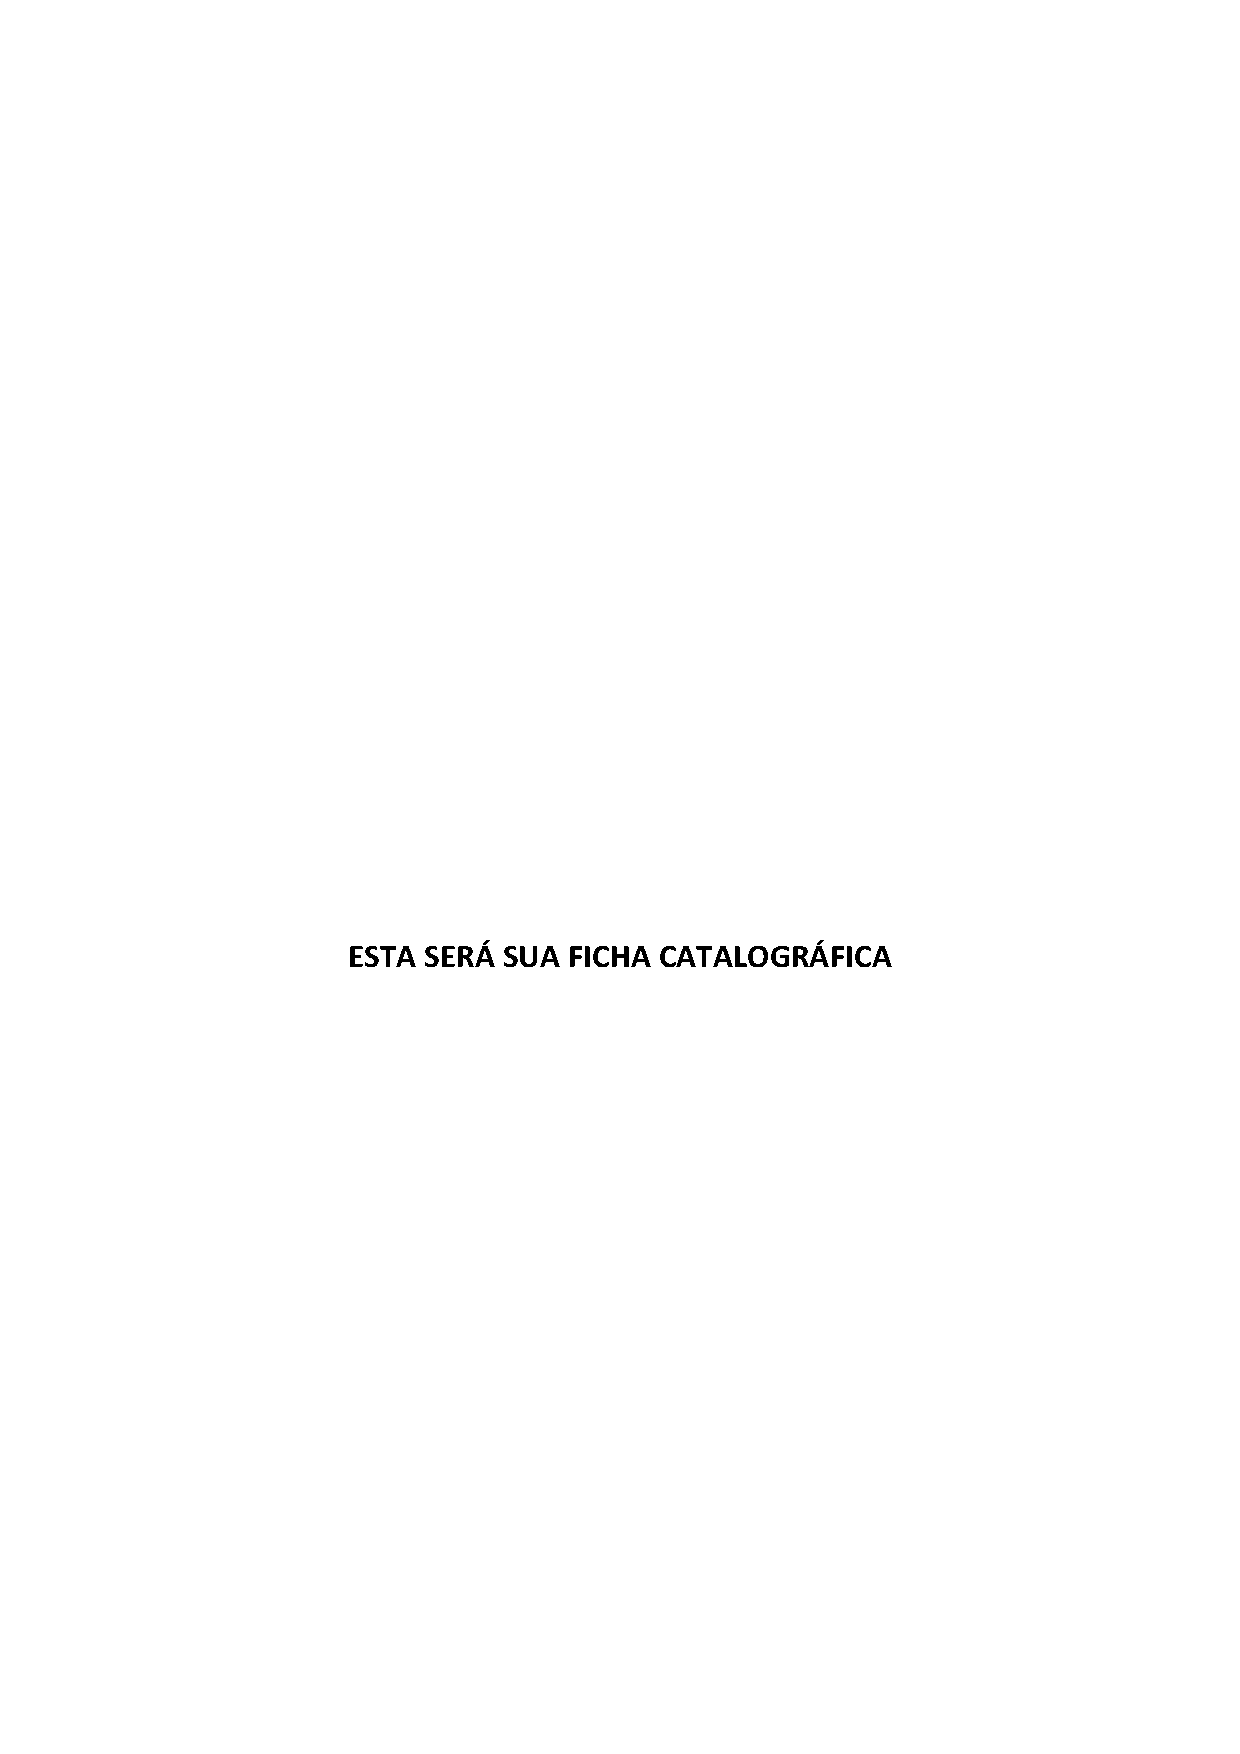
\includepdf[pages=-]{anexos/ficha.pdf}

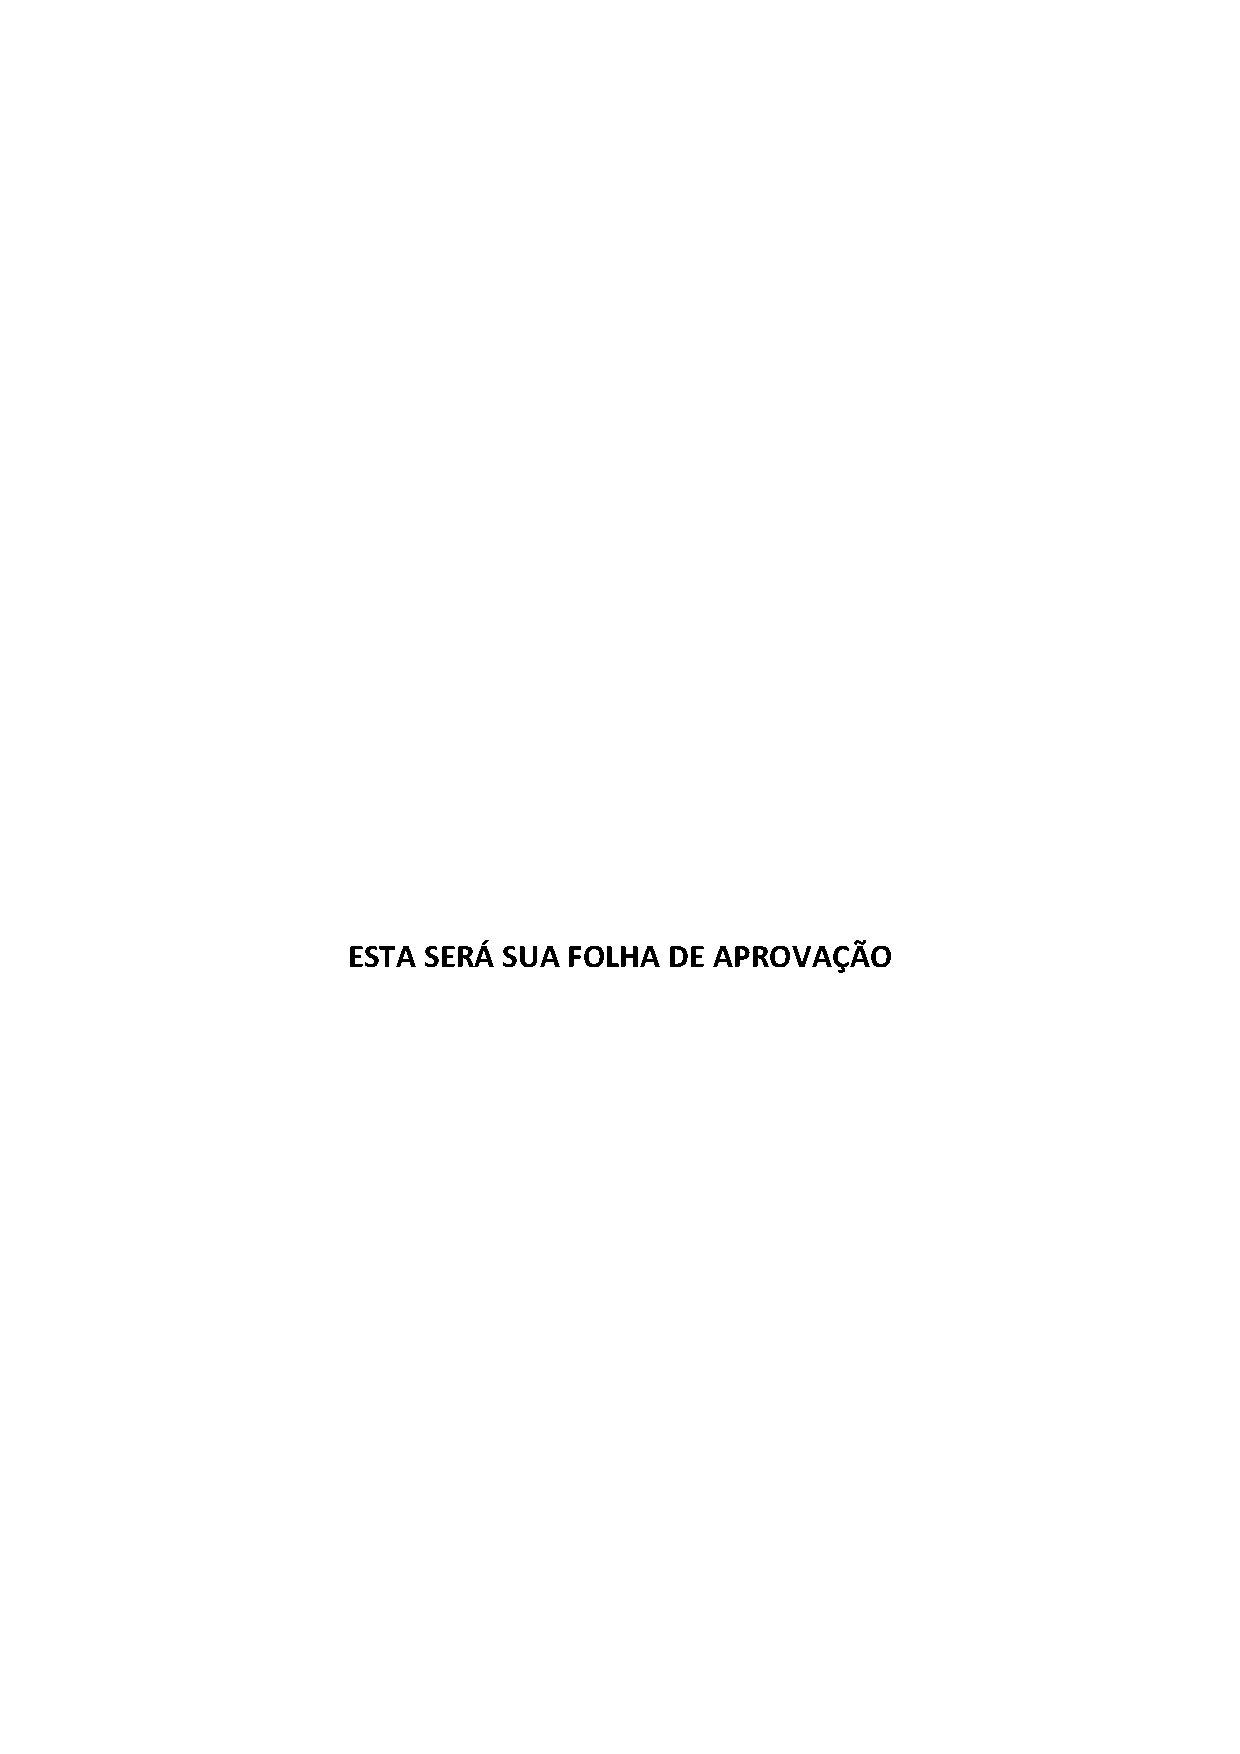
\includepdf[pages=-]{anexos/aprovacao.pdf}

\setlength{\ABNTEXsignwidth}{12cm}

%--------------------------------------------------------------------------------
% Está comentado pelo mesmo motivo da ficha catalográfica
%--------------------------------------------------------------------------------
%\begin{folhadeaprovacao}
%	\begin{center}
%	    {\ABNTEXchapterfont\bfseries\large\imprimirinstituicao}
%	    \vspace*{\fill}
%
%	    {\ABNTEXchapterfont\bfseries\large FOLHA DE APROVAÇÃO}
%	    \vspace*{\fill}
%
%	    {\ABNTEXchapterfont\bfseries\large\imprimirautor}
%
%	    \vspace*{\fill}\vspace*{\fill}
%	    {\ABNTEXchapterfont\bfseries\large\imprimirtitulo}
%	    \vspace*{\fill}
%
%	    {\hspace{.45\textwidth}
%		\begin{minipage}{.5\textwidth}
%			\SingleSpacing
%			\ABNTEXchapterfont\imprimirpreambulo \\ \\
%
%			{\ABNTEXchapterfont\imprimirorientadorRotulo~\imprimirorientador\par}
%			{\ABNTEXchapterfont\imprimircoorientadorRotulo~\imprimircoorientador\par}
%
%		\end{minipage}%
%	    \vspace*{\fill}}
%	\end{center}
%
%	\vspace*{\fill}
%
%	\begin{center}
%			 \ABNTEXchapterfont\large Aprovado em: \_\_\_\_ de \_\_\_\_ de 2017
%	\end{center}

%	\vspace*{\fill}

%	\begin{center}
%			 \ABNTEXchapterfont\bfseries\large Banca Examinadora
%	\end{center}
%
%   \ABNTEXchapterfont\assinatura{Fábio Nelson de Sousa Pereira, Mestre, Universidade Federal do Vale do São Francisco}
%	\ABNTEXchapterfont\assinatura{Jorge Luis Cavalcanti Ramos, Doutor, Universidade Federal do vale do São Francisco}
%  \ABNTEXchapterfont\assinatura{Ricardo Argenton Ramos, Doutor, Universidade Federal do Vale do São Francisco}
%	 \vspace*{\fill}


%\end{folhadeaprovacao}

%--------------------------------------------------------------------------------
% Insere a epígrafe
%--------------------------------------------------------------------------------
\newpage
\vspace*{\fill}
\begin{flushright}
		\textit{“A persistência é o caminho do êxito.”}
		\textbf{Charles Chaplin}
\end{flushright}

%--------------------------------------------------------------------------------
% Seção de agradecimentos
%--------------------------------------------------------------------------------
\begin{agradecimentos}

Agradeço a mim, por não desistir;

Agradeço a Deus, por me dar forças;

Ao meu orientador Professor Mestre e em breve Doutor Juracy Magalhães, compreensivo e paciente, me deu as ferramentas para chegar ate aqui.

Agradeço também aos meus pais, meus irmãos e família, que sempre investiram em mim e confiaram no meu potencial. Agradeço à minha namorada que tanto me incentivou e acreditou em mim. Também quero agradecer aos amigos e colegas que forneceram bons momentos de descontração.

Fico feliz por ter boas pessoas ao meu redor que querem me ver vencendo os desafios da vida! Gratidão.


\end{agradecimentos}

%--------------------------------------------------------------------------------
% Insere a segunda epígrafe
%--------------------------------------------------------------------------------
\begin{epigrafe}
    \vspace*{\fill}
	\begin{flushright}
		Se pude enxergar a tão grande distância, foi subindo nos ombros de gigantes.\\
		 \vspace{\baselineskip}
		\textbf{Isaac Newton}\\
		\textbf{Carta à Robert Hooke, 1676}
	\end{flushright}
\end{epigrafe}



%--------------------------------------------------------------------------------
% Seção de resumos
%--------------------------------------------------------------------------------
% resumo em português
\setlength{\absparsep}{18pt} % ajusta o espaçamento dos parágrafos do resumo
\begin{resumo}

     O estudo da modelagem e simulação do manipulador robótico EEZYBotArm através das ferramentas CoppeliaSim e Robotics Toolbox para Phython (RTB) envolve a cultura Maker, que está firmemente estabelecida e cresce impulsionada pela filosofia do "faça-você-mesmo", e que entre os projetos frequentes nesse movimento, destacam-se os braços robóticos. O propósito deste estudo é realizar a modelagem e simulação de um manipulador robótico fruto da cultura Maker utilizando as ferramentas CoppeliaSim e Robotics Toolbox. Esses manipuladores apresentam várias configurações, incluindo os antropomórficos com geometria em paralelogramo, caracterizados por cadeias fechadas, arquitetura que proporciona alta capacidade de carga, precisão nos movimentos e mantém o efetuador sempre paralelo ao solo, vantajoso para tarefas de paletização. Além disso, no desenvolvimento de manipuladores robóticos, a análise cinemática é de suma importância. A utilização de ferramentas computacionais como simuladores e bibliotecas de ferramentas (toolboxes) torna-se essencial para modelar, visualizar e calcular a cinemática (e dinâmica), particularmente no contexto de braços robóticos com geometria em paralelogramo. Para isso, o modelo virtual do protótipo foi construído no CoppeliaSim, e no RTB foi proposto analisar cineticamente esse manipulador de cadeia fechada para computar os ângulos de junta, estabelecendo comunicação entre essas duas ferramentas para visualizar o resultado no modelo virtual. Ao final deste trabalho, a adoção de um modelo amador e sua modelagem no ambiente de simulação CoppeliaSim e a subsequente análise da cinemática inversa com uso de ferramentas e bibliotecas em Python (uma linguagem de programação) foi bem sucedida, oferecendo esclarecimentos valiosos para o desenvolvimento de modelos semelhantes, e também facilitando a implementação desses modelos em contextos acadêmicos e educacionais, promovendo uma maior interação com a robótica. 
	

 \textbf{Palavras-chave}: \textit{Robótica. Simulação. Modelagem. CoppeliaSim. Manipulador Robótico. Cadeia fechada.}

\end{resumo}

%---------------------------------------------------------------------------------
% resumo em inglês
\begin{resumo}[Abstract]
\begin{otherlanguage*}{english}

	The study of the modeling and simulation of the EEZYBotArm robotic manipulator using the CoppeliaSim and Robotics Toolbox for Phython (RTB) tools involves the Maker culture, which is firmly established and growing, driven by the "do-it-yourself" philosophy, and among the frequent projects in this movement, robotic arms stand out. The purpose of this study is to model and simulate a robotic manipulator resulting from the Maker culture using the CoppeliaSim and Robotics Toolbox tools. These manipulators come in various configurations, including anthropomorphic ones with parallelogram geometry, characterized by closed chains, an architecture that provides high load capacity, precision in movements and keeps the effector always parallel to the ground, which is advantageous for palletizing tasks. Furthermore, in the development of robotic manipulators, kinematic analysis is of utmost importance. The use of computational tools such as simulators and toolboxes is essential for modeling, visualizing and calculating kinematics (and dynamics), particularly in the context of robotic arms with parallelogram geometry. To this end, the virtual model of the prototype was built in CoppeliaSim, and in RTB it was proposed to kinetically analyze this closed-chain manipulator to compute the joint angles, establishing communication between these two tools to visualize the result in the virtual model. At the end of this work, the adoption of an amateur model and its modeling in the CoppeliaSim simulation environment and the subsequent analysis of the inverse kinematics using tools and libraries in Python (a programming language) was successful, offering valuable insights for the development of similar models, and also facilitating the implementation of these models in academic and educational contexts, promoting greater interaction with robotics. 
	

	\vspace{\onelineskip}

	\noindent
	\textbf{Palavras-chave}: \textit{Robotics. Simulation. Modeling. CoppeliaSim. Robotic manipulator. Closed chain.}

\end{otherlanguage*}
\end{resumo}


%---------------------------------------------------------------------------------
% Insere lista de ilustrações
%---------------------------------------------------------------------------------
\begin{KeepFromToc} % Este comando evita que todas as seções dentro dele de apareçam no sumário
\pdfbookmark[0]{\listfigurename}{lof}
\listoffigures
%\addcontentsline{toc}{chapter}{Lista de Figuras}
\cleardoublepage


%---------------------------------------------------------------------------------
% Insere lista de tabelas
%---------------------------------------------------------------------------------
\pdfbookmark[0]{\listtablename}{lot}
\listoftables
\cleardoublepage

%---------------------------------------------------------------------------------
% Insere lista de quadros
%---------------------------------------------------------------------------------
%\pdfbookmark[0]{\listofquadrosname}{loq}
%\listofquadros*
%\cleardoublepage

%---------------------------------------------------------------------------------
% Ajusta lista de código - alterar de figures para códigos - by @Gabrielr2508
%---------------------------------------------------------------------------------
\makeatletter
\let\l@listing\l@figure
\def\newfloat@listoflisting@hook{\let\figurename\listingname}
\makeatother

%---------------------------------------------------------------------------------
% Insere lista de códigos - by @leolleocomp
%---------------------------------------------------------------------------------
\listoflistings


%---------------------------------------------------------------------------------
% Insere lista de abreviaturas e siglas
%---------------------------------------------------------------------------------
\begin{siglas}
	\item[DIY]       Do it yourself
    \item[DH]		 Denavit-Hartenberg
    \item[MDH]		 Modified Denavit-Hartenberg
    \item[RTB]		 Robotics Toolbox
    \item[ROS]       Robot Operating System
    \item[VANTs]     Veículos Aéreos Não Tripulados
	
\end{siglas}
\end{KeepFromToc}

%---------------------------------------------------------------------------------
% Insere o sumario
%---------------------------------------------------------------------------------
\pdfbookmark[0]{\contentsname}{toc}
\tableofcontents*
\cleardoublepage




	\textual
		\pagestyle{simple}
		%--------------------------------------------------------------------------------------
% Este arquivo contém a sua introdução, objetivos e organização do trabalho
%--------------------------------------------------------------------------------------2\chapter{Introdução}
\chapter{Introdução}

A palavra robô tem origem tcheca e significa servidão, aplicada primeiramente numa peça de  teatro de 1920 \cite{Spong2020}. Desde então seu significado ampliou-se, muito se desenvolveu e grandes investimentos foram feitos para que em 1961 o primeiro manipulador robótico fosse lançado, Unimate, por George Devol \cite{Granatyr2017a}.

Os robôs então tiveram grande impacto na sociedade. Hoje os números só aumentam: são mais de 3 milhões de robôs operando em fábricas, com bilhões investidos. Dados da revista “2021 World Robot Report” \cite{Heer2021a}, da Federação Internacional de Robótica, indicam aumento de 10\% de novas unidades instaladas no ano de 2021, um dos melhores anos desde 2018, isso após a pandemia, como mostra a figura \ref{img:figura1.jpg}.

\imagem{0.2}{figura1.jpg}{Novas instalações de robôs industriais por ano.}{\citeonline{Heer2021a}}

Na literatura, robôs fascinam e fazem a imaginação correr. Levados por esse sentimento, pessoas ao redor do mundo  se propõem a desenvolver projetos caseiros dos mais diversos tipos, incluindo robôs e manipuladores robóticos. Essa é a cultura maker, uma subcultura da cultura do DIY ( Do It Yourself), o faça você mesmo, porém a cultura maker é voltada para projetos que envolvem tecnologia, abrangendo diversas áreas do conhecimento, como física, mecânica, eletrônica, engenharia e claro, robótica. \cite{Marini2019a}

Se apropriando desses dois conceitos, de manipuladores robóticos e o desenvolvimento do conhecimento por meio da cultura maker, esse trabalho se propõe a expandir um projeto tido como amador, compartilhado num repositório de entusiastas da cultura maker, e analisar sua cinemática.

Um modelo que tem destaque é o braço robótico com geometria do paralelogramo. Muitos projetos amadores possuem essa estrutura, que também tem grande espaço em uso profissional, seja na indústria ou mesmo em operações médicas. Esse tipo de configuração permite que a ponta do braço robótico, onde se posiciona a sua ferramenta, sempre tenha uma orientação constante, usualmente paralela ao chão, sendo grande vantagem em aplicações industriais.

Ao combinar o CoppeliaSim e o Robotics Toolbox for Python, esta pesquisa visa proporcionar uma abordagem integrada e abrangente para a simulação e análise do manipulador do tipo braço robótico articulado com geometria em paralelogramo,  permitindo uma melhor compreensão do comportamento desse tipo de robô e enriquecendo o conjunto de recursos disponíveis para a comunidade acadêmica e o estudo da robótica.

\section{Definição do Problema}

A cultura maker proporciona a difusão e interesse por temas tecnológicos, como a robótica, uma área que é de grande interesse capital e de contínuo desenvolvimento. No mundo amador, projetos que envolvem braços robóticos com geometria em paralelo são bastante populares. As indústrias têm interesse nesse tipo de braço robótico, esses com geometria em paralelo, pois possuem características interessantes ao tipo de função que executam \cite{Siciliano2009}.

Dito isso, analisar um projeto dito como amador da cultura maker de um braços robótico com geometria em paralelo, aplicando conceitos acadêmicos e ferramentas de simulação para determinar funções de juntas é um grande desafio. Esse tipo de geometria é mais complexa de se analisar e controlar por possuir juntas passivas e ativas, destacando a importância que esse trabalho carrega não somente em termos educacionais, mas também no âmbito financeiro. Do ponto de vista educacional, o projeto de análise, modelagem e simulação de braços robóticos com geometria em paralelo usados em paletização, especificamente, ainda não é tão comum e debatido.


\section{Objetivos}

\subsection{Objetivo Geral} 

O objetivo deste trabalho é modelar e simular o modelo de braço robótico de geometria em paralelo que possui quatro juntas ativas, oito juntas passivas e três cadeias fechadas na ferramenta CoppeliaSim, um ambiente de simulação completo e gratuito para estudantes; e por meio da ferramenta Robotics Toolbox for Python, obter ângulos de junta para esse modelo utilizando suas funções nativas de cálculo de cinemática inversa de forma explícita, pois o CoppeliaSim encapsula as funcionalidades de cinemática.

\subsection{Objetivos específicos}

\begin{itemize}
	\item Estudar os conceitos básicos de robótica, como representação de orientação e posição no plano 2D e 3D; braços robóticos e suas geometrias; Cinemática direta e inversa dos braços robóticos;
    \item Em posse dos arquivos CAD do manipulador de interesse, modelar a hierarquia de elos e juntas no simulador CoppeliaSim, tendo em vista a geometria em paralelo dessa manipulador;
    \item Fazer a comunicação entre as ferramentas CoppeliaSim e Robotic Toolbox para Python;
	\item No RTB, obter ângulos de juntas por meio da cinemática inversa;
\end{itemize}

\section{Organização do trabalho}
 
O Capítulo 1 apresenta uma breve introdução da robótica e suas aplicações, incluindo os manipuladores robóticos e destaca a importância da modelagem cinemática dos manipuladores. Também menciona os braços robóticos com geometria em paralelogramo e cadeias fechadas. Aborda as ferramentas de simulação e modelagem CoppeiaSim e Robotics Toolbox for python, e também a definição do problema e objetivos deste trabalho.
O Capítulo 2 trata, essencialmente, da revisão bibliográfica do trabalho que contém conceitos úteis relacionados a modelagem e simulação em ambientes como o CoppeliaSim, trabalhos relacionados ao tema de modelagem em ambientes virtuais e conceitos relacionados aos manipuladores robóticos, procedimentos necessários para a obtenção da modelagem cinemática do manipulador. No Capítulo 3 são apresentados as técnicas e os métodos adotados para o desenvolvimento deste trabalho.  Os passos para a modelagem, a comunicação entre as plataformas de trabalho e simulações. No Capítulo 4 apresentam-se os resultados finais e validação dos modelos. Finalmente no Capítulo 5 a conclusão desse trabalho e as propostas para trabalhos futuros.


		
\chapter{Referencial teórico}

\section{Estado da arte}

A modelagem cinemática de robôs com cadeia fechada é uma área de grande relevância na robótica e tem sido objeto de intensa pesquisa nas últimas décadas, principalmente em trabalhos que investigam novas formas de aperfeiçoar o processo de calibragem desses manipuladores. Para calibrar um manipulador, diversas técnicas são utilizadas, mas inicialmente é necessário formular o modelo cinemático do equipamento o que é comum em diversos trabalhos.

Para o modelo cinemático de um manipulador robótico com a presença de geometria em paralelogramo e uma única cadeia fechada, como é o caso do modelo de robô ABB IRB 6660 (Fig. \ref{img:irb6660.jpg}), \citeauthoronline{peng2019} (\citeyear{peng2019}) utilizou a seguinte estratégia: abrir virtualmente essa cadeia, formando-se assim duas novas, a curta e a longa, que é o procedimento explicitado por \citeauthoronline{Siciliano2009} no seu livro Robotics modelling, planning and control (2.9.2). Ele cita outros trabalhos e como essa situação foi abordada, alguns pela cadeia curta e outros pela cadeia longa, chegando a conclusão de que a diferença entre os modelos cinemáticos não fica clara. Após a análise cinemática, fica evidente para o autor que os dois modelos alternativos possuem diferentes parâmetros, mas que por a cadeia curta ter uma estrutura mais simples, foi a cadeia adotada. Ao fim, o trabalho proposto teve maior eficiência computacional com praticamente a mesma precisão e é melhor para a calibragem cinemática em relação ao modelo baseado na cadeia longa.

\imagem{0.5}{irb6660.jpg}{ABB IRB 6660.}{ Adaptado de ABB Robotics}

Outra convenção usada foi na obtenção dos parâmetros de Denavit-Hartenberg (DH) para esse tipo de estrutura fechada. Os parâmetros de DH são obtidos de forma sequencial, frame a frame, mas é violado quando duas juntas consecutivas são paralelas, que é o caso de geometria em paralelogramo. Para contornar esse problema, \citeonline{hayati1983} propôs um modelo de DH modificado (MDH), com a introdução de um novo parâmetro rotacional em relação ao eixo y para descrever as juntas que fazem parte da cadeia fechada.

Essa abordagem foi utilizada por \citeauthoronline{towebb2012} (\citeyear{towebb2012}) no artigo An improved kinematic model for calibration of serial robots having closed-chain mechanisms (Um modelo cinemático aprimorado para calibração de robôs seriais com mecanismos de cadeia fechada em tradução livre) publicado por Cambrige University Press, juntamente com a abordagem citada anteriormente, abrindo  virtualmente a cadeia fechada. Levando em conta um manipulador Comau Smart H4 (Fig. \ref{img:smartH4.png}), esse trabalho propôs um método que melhorou a calibragem da precisão em comparação com o modelo cinemático curto (negligenciando  a estrutura em paralelogramo). Outros trabalhos também usaram a convenção de \citeonline{hayati1983}, como \citeonline{newman2000} e \citeonline{alici2005}.

\imagem{0.5}{smartH4.png}{Comau Smart H4.}{\cite{towebb2012}}

A modelagem da cinemática inversa de um manipulador robótico com três cadeias fechadas, como o EEZYbotARM, foi abordado pelo trabalho de \citeauthoronline{costa2017} (\citeyear{costa2017}). Utilizaram como modelo a ser estudado o protótipo MeArm v0.4, que assim como o EEZYbotARM é um projeto amador disponibilizado na plataforma Thingisverse e que se assemelha com o robô industrial ABB IRB 460 (Fig. \ref{img:figura13.jpg}). Uma consideração importante foi a posição da junta 3 ($\theta_3$), situada no ponto de rotação do elo 3. Porém a junta que ativamente faz esse movimento se localiza no elo 2, e que por meio de uma estrutura em paralelogramo, efetua o movimento do terceiro elo. Abordar o problema dessa maneira facilita o desenvolvimento do modelo geométrico desse manipulador. \citeonline{costa2017} então determinam as funções de junta que informam os valores de $\theta_1$, $\theta_2$ e $\theta_3$ em relação ao ponto (x, y, z).

\imagem{0.5}{figura13.jpg}{ABB IRB 460}{Fonte: ABB Robotics}

O trabalho de \citeauthoronline{gienke2019} (\citeyear{gienke2019}) busca prever e prevenir vibrações de acoplamento em manipuladores que executam usinagem. O modelo cinemático do manipulador ABB IRB 6660 foi feito levando em conta apenas a cadeia curta, pois apenas as juntas ativas e suas engrenagens poderiam causar vibrações, portanto as juntas passivas não foram modeladas.

\subsection{Trabalhos Relacionados ao CoppeliaSim}

O trabalho de  \citeauthoronline{wang2023} (\citeyear{wang2023}) utiliza o ambiente de simulação do CoppeliaSim para desenvolver redes neurais com conexões laterais, a fim de propor transferência externa de aprendizado de máquina para ajudar em novas tarefas. Novos métodos se mostraram eficazes em alcançar transferências de tarefas construindo conexões laterais entre redes neurais totalmente convolucionais, utilizando um modelo de braço robótico já presente no banco de dados do CoppeliaSim, o UR5, um braço robótico serial.

O estudo conduzido por \citeauthoronline{ferro2022} (\citeyear{ferro2022}) se concentra no desenvolvimento de simulações no ambiente CoppeliaSim para um manipulador robótico com geometria de paralelogramo que realiza procedimentos cirúrgicos minuciosos. A arquitetura em paralelogramo oferece a rigidez e precisão necessária para esse tipo de tarefa. Esse trabalho representa uma extensão do estudo anterior realizado por \citeauthoronline{fontanelli2018}  (\citeyear{fontanelli2018}), no qual a simulação cinemática do manipulador foi abordada. O estudo atual propõe estender a análise cinemática para incluir a simulação dinâmica do Kit de Pesquisas da Vinci, se valendo do poderio do CoppeliaSim para inserir informações que mais se aproximam da realidade, validando o sistema de controle desse manipulador, garantindo segurança nas atividades médicas.

\citeauthoronline{pereira} apresentam uma abordagem de simulação usando o CoppeliaSim e ROS (Robot Operating System) para demonstrar como os sensores a laser podem ser usados para localizar, identificar e pegar objetos e transportá-los para um local diferente. Em seu artigo, eles propõem algoritmos para permitir que um robô manipulador móvel navegue em seu ambiente e execute tarefas consideradas simples para humanos, mas complexas para robôs, como pegar pequenos objetos domésticos. O robô simulado consiste em uma base móvel acoplada a um manipulador Mico com seis graus de liberdade, e os algoritmos de controle incluem prevenção de colisões e reconhecimento de objetos. Os autores também discutem o potencial de aplicação dessa abordagem de simulação à robótica do mundo real.

\citeauthoronline{coelho2021}  (\citeyear{coelho2021}) apresentam um estudo sobre a locomoção de hexápodes em ambientes desafiadores usando o CoppeliaSim e o ROS. Sua pesquisa se concentra no uso de sensores de força para controlar as mudanças de fase da marcha de cada membro e se adaptar a novos pontos de apoio. Por meio de experimentos e simulações, eles avaliam a viabilidade desse sistema de controle e seu potencial para melhorar a autonomia dos hexápodes. Suas descobertas têm implicações importantes para o desenvolvimento de robôs hexápodes mais robustos e adaptáveis no futuro. De acordo com \citeauthoronline{coelho2021} (\citeyear{coelho2021}), o uso do CoppeliaSim e do ROS permite a avaliação não apenas do movimento gerado pelo hexápode, mas também do torque exigido pelos atuadores e das forças de interação. Esse software fornece uma estimativa das interações dinâmicas do sistema e pode estimar as possíveis falhas do hexápode durante a navegação. Além disso, ele fornece uma visão do comportamento dos controladores. Os autores observam que poucas pesquisas estudaram a locomoção de hexápodes nesse software, mas seu estudo demonstra seu potencial para avaliar a viabilidade dos controladores de hexápodes e melhorar sua autonomia em ambientes complexos.

\citeauthoronline{wang2022research} (\citeyear{wang2022research}) apresentam uma nova abordagem para o controle de braços robóticos móveis usando o aprendizado por reforço. O método proposto envolve o treinamento do braço robótico para executar uma tarefa específica, como abrir uma porta. Os pesquisadores usaram o CoppeliaSim para construir um ambiente de simulação para o braço robótico móvel e para treinar o algoritmo de aprendizagem por reforço. Isso permitiu que eles testassem a estratégia de controle em um ambiente seguro e controlado antes de aplicá-la a um cenário do mundo real. O controlador do manipulador foi feito em Python e os comandos enviados pela interface RemoteAPI do CoppeliaSim. Os resultados mostraram que o método proposto foi eficaz no controle do braço robótico e pode ser aplicado a uma variedade de cenários, incluindo resgate em ambientes perigosos e inspeção de equipamentos internos. 

 Através da conjunção do CoppeliaSim e do Robotics Toolbox for Python, este estudo busca estabelecer uma abordagem integrada e abrangente na simulação e análise de um braço robótico articulado com geometria em paralelogramo. Até o momento, observa-se uma lacuna na literatura científica quanto à exploração dessa configuração geométrica específica em um contexto simulado através do emprego destas ferramentas particulares.

\subsection{Simulador de Robô CoppeliaSim}

CoppeliaSim é uma ferramenta de simulação que permite aos usuários criar e testar sistemas robóticos virtuais. Possui uma interface amigável que permite aos usuários projetar e simular sistemas de vários robôs com facilidade. O software fornece uma ampla gama de modelos e componentes pré-construídos, tornando fácil para os usuários criar modelos robóticos personalizados. CoppeliaSim também pode simular o comportamento do robô em tempo real, tornando-o uma ferramenta ideal para testar e desenvolver algoritmos de controle \cite{nascimento2019}

O simulador CoppeliaSim se destaca como uma ferramenta amplamente utilizada para fins pedagógicos. Ele oferece um ambiente versátil e escalável para criar simulações em 3D em um curto espaço de tempo. Com sua arquitetura distribuída e baseada em scripts, cada objeto na cena pode ter um script embutido, permitindo operações simultâneas em forma de threads. Além disso, CoppeliaSim oferece diversos exemplos, modelos de robôs, sensores e atuadores para criar e interagir com um mundo virtual em tempo real \cite{Montenegro2022}.

 Diversos trabalhos têm utilizado a plataforma CoppeliaSim, abordando diferentes aplicações na robótica e sistemas multi-agente. Por exemplo, em \citeauthoronline{Obdrzalek2017} (\citeyear{Obdrzalek2017}) é apresentada uma estratégia para a utilização de um sistema multi-agente composto por Veículos Aéreos Não Tripulados (VANTs). Já \citeonline{knoll2017} propõe um esquema de navegação para robôs terrestres utilizando um conjunto de sensores de radiofrequência. Em \citeauthoronline{Tanberk2017} (\citeyear{Tanberk2017}) o simulador CoppeliaSim é empregado para testar um robô capaz de interpretar dados provenientes de um sensor Kinect, a fim de tomar decisões para a movimentação de peças em um jogo de xadrez. 

 O CoppeliaSim oferece uma interface de programação robusta e versátil, permitindo a criação de scripts personalizados para controle, análise e interação dos robôs e objetos no ambiente virtual. A ferramenta também suporta a integração de algoritmos de controle, proporcionando uma ampla gama de opções para experimentos e validações. A facilidade de uso do CoppeliaSim é destacada por sua interface gráfica intuitiva, que possibilita a configuração e visualização detalhada dos modelos robóticos e ambientes simulados. Além disso, o simulador oferece um extenso conjunto de recursos, como bibliotecas de modelos de robôs, sensores e atuadores, acelerando o processo de desenvolvimento de simulações. A possibilidade de comunicação em tempo real com as bibliotecas de programação mais populares, bem como com plataformas de hardware real, torna o CoppeliaSim uma escolha versátil para a validação e testes de algoritmos de controle em ambientes virtuais antes da implementação em robôs reais. Na versão mais recente, modulos de cinemática direta e inversa já vêm instalados. 

\subsection{Robotics Toolbox para Python}
O Robotics Toolbox para Python é uma biblioteca de funções e classes que fornece uma ampla gama de ferramentas para pesquisa e educação em robótica. Ele permite que os usuários criem e manipulem modelos robóticos, realizem análises cinemáticas e dinâmicas e simulem o comportamento do robô. \citeonline{haviland2023dkt1} propõem um tutorial em duas partes abordando a cinemática de robôs manipuladores, conceito fundamental no estudo e uso de braços robóticos. A caixa de ferramentas também fornece suporte para vários sensores e atuadores comumente usados em robótica, tornando possível criar simulações realistas e precisas de sistemas robóticos \cite{rtb2021}.

A biblioteca também disponibiliza recursos avançados para o planejamento de trajetórias, tornando possível simular e testar estratégias de movimentação em robôs móveis e manipuladores. Além disso, a integração do Robotics Toolbox for Python com outras bibliotecas populares de aprendizado de máquina e visão computacional permite o desenvolvimento de soluções mais abrangentes e inteligentes em aplicações de robótica \cite{rtb2021}. 

Quando usados em conjunto, CoppeliaSim e Robotics Toolbox para Python criam uma plataforma poderosa para simulação e modelagem de robótica. Os usuários podem projetar sistemas robóticos usando o Robotics Toolbox para Python e, em seguida, simular seu comportamento em CoppeliaSim. O Robotics Toolbox para Python também pode gerar as entradas necessárias para a simulação e analisar os dados de saída.


\section{Manipuladores Robóticos}

A globalização e abertura de mercado fomentou um aumento na produtividade, estimulando o lucro e a agilidade, e claro, reduzindo os custos. Para se manter competitivos, novas técnicas de produção foram pensadas ao longo das últimas décadas. Visando também uma uniformidade na produção e garantias na qualidade dos produtos, a indústria cada vez mais vem inserindo formas de automação e a utilização de robôs manipuladores, principalmente em tarefas pré-determinadas e repetitivas. Nesse cenário, manipuladores robóticos se mostram como a ferramenta ideal que propõe precisão e alta velocidade \cite{Vale2011}.

Um manipulador robótico é um dispositivo controlado por software, com uma
finalidade específica para os diversos tipos de processos automatizados. Muitas vezes se utilizam de sensores para auxiliar na movimentação e dar feedback ao controlador. Desde o primeiro manipulador patenteado por George Devol em 1954, mostrado na figura \ref{img:figura2.png}, até os dias de hoje, a robótica abraçou várias áreas do conhecimento como as engenharias mecânica, elétrica e da computação. Se desenvolveu impulsionada pela exploração subaquática e espacial, medicina e principalmente na indústria \cite{Lopes2002}.

\imagem{0.3}{figura2.png}{Unimate robot, por George Devol, 1961.}{\citeonline{IEEE2018}}

\subsection{Estrutura}

Atualmente muito utilizados nas indústrias, esses equipamentos são máquinas de grande investimento tecnológico. Geralmente são manipuladores do tipo antropomórficos, pois assemelham-se a um braço humano. Posicionados de forma fixa, possuem juntas flexíveis, braços e tronco. Na linguagem utilizada nesse trabalho, o tronco é a base do manipulador, geralmente dita como referencial do sistema e fixa no solo. Os braços são os elos (na literatura em inglês, links), conectados por juntas flexíveis (joints), e a última junta, o punho. O punho é responsável pela orientação final da extremidade do braço. Na extremidade então é fixada a ferramenta ou dispositivo o qual realiza a tarefa desejada. A ferramenta chamamos de órgão terminal. \cite{Spong2020}



\subsubsection{Juntas}

Segundo \cite{Santos2004} as juntas se dividem em tipos únicos para cada finalidade. Podem ser do tipo:
\begin{itemize}
	\item Prismática (P): essas movem-se em linha reta, compostas por duas hastes que
	deslizam entre si (Fig. \ref{img:subfigura1});
        
	\item Rotacional (R): as juntas rotacionais giram em torno de uma linha imaginária, o eixo
	de rotação (Fig. \ref{img:subfigura2}). Comumente, e nesse trabalho,
	estabelecemos que as juntas rotacionais giram em torno do eixo z;

	\item Esférica (S): as juntas esféricas funcionam como como uma combinação de três juntas
	rotacionais, tendo a liberdade de girar em torno dos três eixos, ilustrado \ref{img:subfigura3}.

	\item Cilíndrica ou Revolvente (V): basicamente composta por duas juntas, uma rotacional
	e outra prismática (Fig. \ref{img:subfigura4});

	\item Planar: formada por duas juntas prismáticas, permitindo movimentos em duas
	direções (Fig. \ref{img:subfigura5});

	\item Parafuso ou Torcional (T): é constituída por um parafuso e uma porca. Tem
	movimento semelhante ao da junta prismática, porém com movimento no eixo
	central, como ilustrado na figura \ref{img:subfigura6}.		\

\end{itemize}

\begin{figure}[!htb]
\centering
    \caption{\label{img:figura1} Tipos de Juntas}
    \subcaptionbox{\label{img:subfigura1} Junta prismática.}{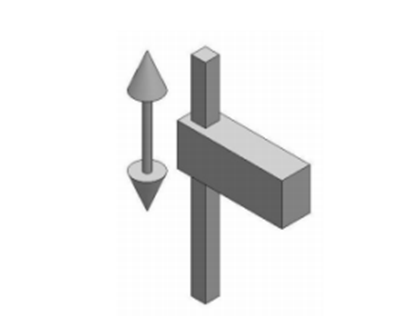
\includegraphics[scale=.55]{img/figura3.png}}
    \subcaptionbox{\label{img:subfigura2} Junta rotacional.}{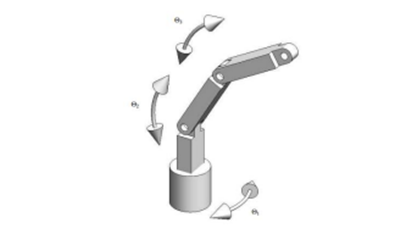
\includegraphics[scale=.55]{img/figura4.png}}
    \subcaptionbox{\label{img:subfigura3} Junta esférica.}{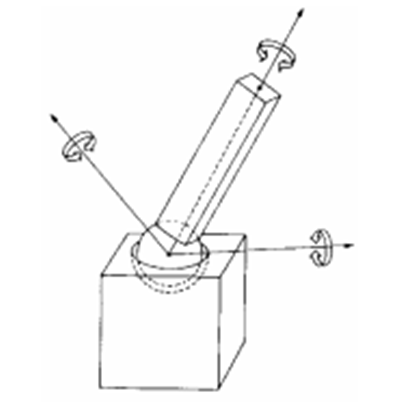
\includegraphics[scale=.55]{img/figura5.png}}
    \subcaptionbox{\label{img:subfigura4} Junta revolvente.}{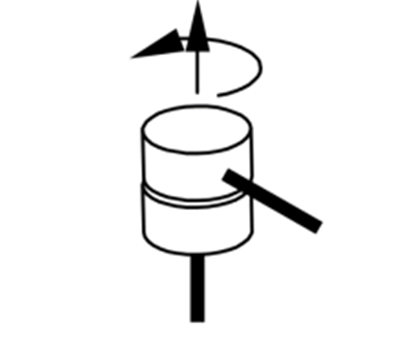
\includegraphics[scale=.55]{img/figura6.png}}
    \subcaptionbox{\label{img:subfigura5} Junta planar.}{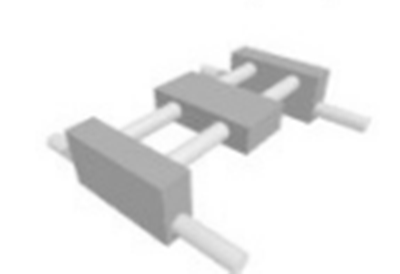
\includegraphics[scale=.55]{img/figura7.png}}
    \subcaptionbox{\label{img:subfigura6} Junta torcinal.}{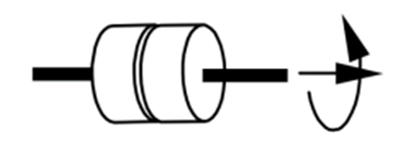
\includegraphics[scale=.55]{img/figura8.png}}
    \vspace{1.0em}
    \legend{\textbf{Fonte:} Adaptado de \citeonline{Santos2004}}
\label{fig:dag}
\end{figure}

As juntas do manipulador conferem diversos graus de liberdade - gdl - (Na literatura em inglês, Degrees of Freedom). E são os gdl que determinam os movimentos do manipulador no espaço tridimensional \cite{Santos2004}.

\subsubsection{Graus de Libertade (gdl) e graus de mobilidade (gdm)}

Os graus de liberdade definem o número total de movimentos independentes que o manipulador pode executar.

Diferentemente, os graus de mobilidade estão associados ao número de juntas existentes.

Um exemplo para demonstrar a diferença entre eles são os tripes, como esses usados por fotógrafos.  Em cada pé temos várias juntas prismáticas que permitem o movimento ao longo do mesmo eixo. Se em cada tripé houver três juntas, temos um tripé com 3 graus de liberdade mas 9 graus de mobilidade (3 gdl * 3 pés do tripé) \cite{Santos2004}.

\subsubsection{Tipos de configurações}

Como dito anteriormente, um manipulador robótico do tipo antropomórfico é formado por base, braço e órgão terminal. É a base que sustenta todo o manipulador, de onde o braço se movimenta, posicionando o punho no espaço. O punho então orienta o órgão terminal que por fim realiza sua função.

A configuração do manipulador é dada pelos tipos de juntas que ele possui. Então temos alguns tipos comuns de robôs manipuladores:

\begin{itemize}
	\item Manipulador cartesiano (PPP): é um manipulador composto por três juntas prismáticas - daí a representação das letras PPP. Consegue movimentar seu órgão terminal nas direções (x, y, z) do plano cartesiano. Na figura \ref{img:subfigura7} pode-se ver um exemplo de manipulador cartesiano, o robô Epson. Então as variáveis das juntas são coordenadas cartesianas do órgão terminal em relação a base.		\

	\item Manipulador Cilíndrico (RPP): o manipulador cilíndrico é formado por uma primeira junta rotacional na base e a segunda e terceira juntas são prismáticas, recebendo esse nome porque as variáveis das juntas são as coordenadas cilíndricas do órgão terminal em relação a base. Na figura \ref{img:subfigura8} é exemplificado o robô cilíndrico Seiko RT3300.

	\item Manipulador Esférico (RRP): formado pela primeira junta rotacional em relação a
	base, a segunda também rotacional e a terceira junta prismática. Todas as três juntas
	são dispostas de modo que seus eixos de trabalho são perpendiculares entre si. O
	termo manipulador esférico se justifica porque coordenadas esféricas definem a
	posição do órgão terminal em relação à origem. A origem nesse caso não é na base,
	mas na intersecção dos três eixos z (eixo o qual a junta rotaciona em torno). Na figura
	\ref{img:subfigura9} temos o Stanford Arm, um dos mais conhecidos robôs esféricos.
		
	\item Manipulador SCARA (RRP): : O acrônimo SCARA se traduz como Robô Articulado
	Seletivo Compatível para Montagem (Selective Compliant Articulated Robot for
	Assembly), exemplificado na figura \ref{img:subfigura10}. É um manipulador bastante popular, e como o
	nome sugere, ideal para operações de montagem, e se difere em relação ao manipulador
	esférico na orientação dos eixos z das juntas. Aqui os três eixos $z_1$, $z_2$ e $z_3$ são
	paralelos entre si.

	\item Manipulador Articulado (RRR): é o manipulador chamado também de
	antropomórfico ou manipulador de revolução. Nele é muito usada uma configuração
	de ligação em paralelogramo. Nesse arranjo temos três juntas rotacionais. A segunda e
	terceira juntas possuem seus eixos de rotação $z_2$ e $z_3$ paralelos entre si. E $z_2$ e $z_3$ são
	perpendiculares ao eixo de rotação $z_1$ da primeira junta. Na figura \ref{img:subfigura11} observa-se o robô
	articulado ABB IRB 460, que possui uma grande área de movimento e se mantém
	compacto. Esse arranjo de ligação em paralelogramo possui algumas vantagens, como
	o fato de que o atuador da terceira junta poder ficar localizado no primeiro elo. Dessa
	forma, o peso do motor fica no primeiro elo, e o segundo e terceiro elo ficam mais
	leves, sobrando mais potencia para realizar a tarefa em si. Por isso são muito usados em operações com carga útil pesada \cite{Siciliano2009}. E ainda, esse arranjo é
	mais simples de se analisar sua dinâmica, que se traduz em vantagem para etapas de planejamento de trajetória e o desenvolvimento do controlador \cite{Spong2020}.
	
\end{itemize}

\subsubsection{Braços robóticos com geometria do paralelogramo}
.

Uma das configurações dos manipuladores robóticos é do tipo paralelo. Diferente da configuração serial, a configuração do tipo paralelo possui duas ou mais cadeias cinemáticas fechadas, ligando a base ao órgão efetuador na ponta \cite{Siciliano2009}. Esse tipo de configuração garante mais firmeza e rigidez, dessa forma sendo mais preciso que configurações de cadeia aberta.

Manipuladores antropomórficos, como o braço robótico, mais especificamente do tipo “cotovelo ", possuem também cadeias cinemáticas fechadas em geometrias de paralelogramo. Além da rigidez, esse tipo de configuração também reduz a quantidade de espaço necessário para o braço. Isso porque a geometria em paralelogramo permite que o braço se estenda verticalmente, sem exigir espaço adicional horizontalmente.

Braços robóticos com geometria de paralelogramo são frequentemente utilizados em tarefas de montagem e tarefas do tipo \textit{pick and place}, como posicionar produtos em caixas ou paletes (paletização). Da mesma forma, são utilizados em tarefas de pintura e soldagem. Por sua capacidade de alta precisão, também são utilizados em procedimentos médicos, como posicionar instrumentos cirúrgicos com precisão e delicadeza.
\begin{figure}[!htbp]
\centering
    \caption{\label{img:figura2} Configurações do manipulador}
    \subcaptionbox{\label{img:subfigura7} Robô cartesiano da Epson.}{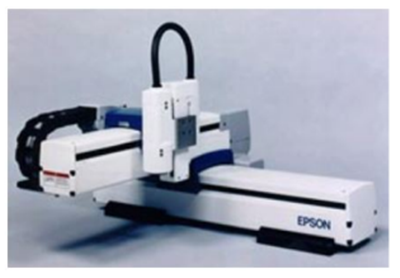
\includegraphics[scale=.6]{img/figura9.png}}
    \subcaptionbox{\label{img:subfigura8} Robô cilíndrico Seiko RT3300.}{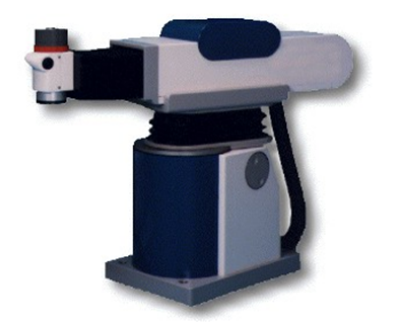
\includegraphics[scale=.6]{img/figura10.png}}
    \subcaptionbox{\label{img:subfigura9} Stanford Arm, manipulador esférico.}{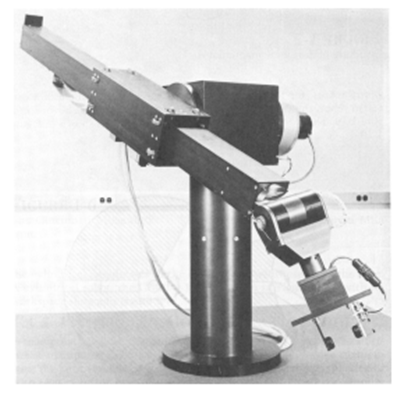
\includegraphics[scale=.6]{img/figura11.png}}
    \subcaptionbox{\label{img:subfigura10} Robô SCARA Epson E2L653S.}{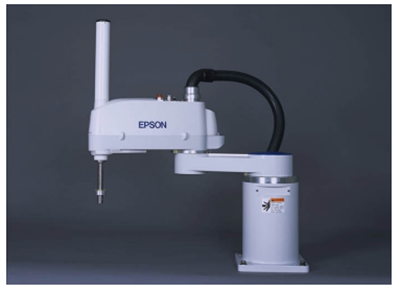
\includegraphics[scale=.6]{img/figura12.png}}
    \subcaptionbox{\label{img:subfigura11} Robô articulado com geometria em paralelogramo ABB IRB 460.}{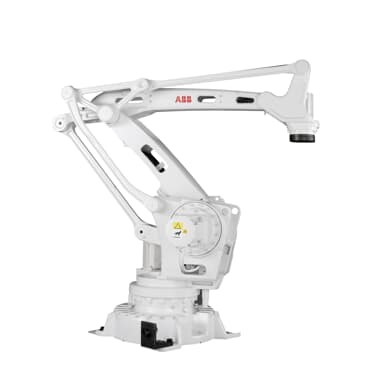
\includegraphics[scale=.6]{img/figura13.jpg}}
    \vspace{1.5em}
    \legend{\textbf{Fonte:} \citeonline{Spong2020}}
\label{fig:dag}
\end{figure}
\pagebreak

\subsection{Cinemática Direta}

Esses elos ligados por juntas então formam uma cadeia cinemática. Imagine um cenário onde queremos fazer o órgão terminal sair da posição inicial home, ir até um ponto A no espaço, percorrer um caminho S até chegar ao ponto B. São vários problemas a serem resolvidos a fim de conseguir executar tal ação.

A cinemática direta descreve a posição do órgão terminal (x, y, z) com base nos parâmetros dos ângulos das juntas que formam o braço robótico $\theta_1, \theta_2, \theta_3$. Dessa forma, a posição e orientação do órgão terminal pode ser expressa por uma função das variáveis conjuntas. Comumente o manipulador consegue informar sua posição com base nos ângulos das juntas por meio de sensores (encoders nos servo-motores que indicam sua angulação).

Para fazer a modelagem da cinemática direta utiliza-se o método de Denavit-Hartenberg (DH)  para obtenção dos parâmetros envolvidos. Os parâmetros de DH fazem parte de uma convenção popular, introduzida em 1955, na qual uma matriz de transformação homogênea é descrita por meio de quatro parâmetros, e que leva as coordenadas do $frame_i$ para o $frame_i+1$ \cite{Spong2020}.

\subsubsection{Convenção de Denavit-Hartenberg}

Sendo um manipulador formado por um conjunto de elos conectados por juntas formando uma cadeia cinemática, é necessário definir a identificação de cada componente. Os elos, então, são numerados a partir da base, sendo o primeiro o elo 0. Quanto às juntas, a primeira é a número 1. Dessa forma, em qualquer configuração do manipulador, a junta $i$ conecta os dois elos, $i-1$ e $i$ \citeonline{Spong2020}.

O método de DH consiste em três etapas principais: definir os sistemas de coordenadas, definir os parâmetros e então construir a matriz de transformação homogênea.

\begin{enumerate}
	\item Sistema de coordenadas: As escolhas de sistema de coordenadas podem variar, porém todas elas chegam ao mesmo resultado para uma dada estrutura. Aqui usaremos o eixo $z_i$ ao longo do eixo da junta $i+1$, como mostra a ilustração \ref{img:figura14.png}.
	\item Definição dos Parâmetros: A figura \ref{img:figura14.png} exemplifica dois elos conectados por uma junta. Daí obtém-se os quatro parâmetros para a convenção DH dessa junta e os dois elos, definindo o comportamento dos desses. São eles:
	
		\begin{itemize}
			\item $a_i = tamanho\:do\:elo;$
			\item $d_i = deslocamento\:do\:elo;$
			\item $\alpha_i = giro\:do\:elo;$
			\item $\theta_i =  \hat{a}ngulo\:da\:junta. $
		\end{itemize}
	
	\imagem{.5}{figura14.png}{Parâmetros de Denavit-Hartenberg.}{\citeonline{Siciliano2009}}
	
	\item  Matriz de Transformação Homogênea: Com os parâmetros definidos, a última etapa é montar a matriz de transformação homogênea. Dos quatro parâmetros, dois estão associados à componente móvel, às juntas. Se a junta for prismática, a variável da junta é o deslocamento di. Se for uma junta rotacional, a variável em questão será $\theta_i$. Os outros dois parâmetros estão associados aos elos, são fixos. A matriz de transformação homogênea é dada por \eqref{eq:1}:

\begin{equation}
	A_i = Rot(z,\theta_1)Trans(a_i, 0, 0)Trans(0, 0, d_i)Rot(x,\alpha_i)
	\label{eq:1}
\end{equation}
		
e a transformação que descreve a cinemática da base em relação ao punho (último frame antes do órgão terminal) é dado por \eqref{eq:2}:

\begin{equation}
	^0T_n = A_0A_1...A_n
	\label{eq:2}
\end{equation}

\end{enumerate}

\subsection{Cinemática Inversa}
A análise da cinemática inversa nos fornece as funções que relacionam a posição Pw do punho (x, y, z), frame o que se posiciona o órgão terminal, com os valores das juntas ($\theta_i$). Pode-se dizer que são
exatamente o inverso das funções que a cinemática direta nos fornece. Simbolicamente dado por \eqref{eq:3},

\begin{align}
	&\vec{r} = \vec{F}(q); \nonumber\\
	&q = \vec{F}^{-1}\vec{(r)}; \vec{F}^{-1} :\Re^n \rightarrow \Re^6
	\label{eq:3}
\end{align}

Graficamente, entende-se como ilustrado em \ref{img:figura15.png}:

	\imagem{1.0}{figura15.png}{Relação entre cinemática inversa e direta.}{ Adaptado de \citeonline{Santos2004}}

Muitas vezes, o problema da cinemática inversa não tem solução. Ou ainda, pode assumir infinitas soluções. Resolver esse problema analiticamente muitas vezes se
mostra uma tarefa onerosa. Alternativamente, adotar métodos numéricos iterativos, mesmo
que sejam menos precisos, pode ser melhor se a cada iteração o método convergir para o
desejado, com base em valores sugeridos para as variáveis.

Métodos como esse utilizam a matriz jacobiana do manipulador. O jacobiano J é
composto pelas derivadas parciais das posições do órgão terminal em relação aos ângulos
das juntas, dado em \eqref{eq:4}. Portanto, dado um deslocamento infinitesimal, o jacobiano expressa a relação entre o deslocamento das juntas e a localização do órgão terminal. Em outras palavras, ao
invés de descrever a posição do órgão terminal, o jacobiano descreve seu movimento\cite{Nilsson2009}.

\begin{equation}
J = \begin{vmatrix}
		\displaystyle
			\frac{\delta x_e}{\theta_1} & \displaystyle ...  & \displaystyle \frac{\delta x_e}{\theta_n} \\ 
		\displaystyle
			\frac{\delta y_e}{\theta_1} & \displaystyle ...  & \displaystyle \frac{\delta y_e}{\theta_n} \\ 
		\displaystyle
			\frac{\delta z_e}{\theta_1} & \displaystyle ...  & \displaystyle \frac{\delta z_e}{\theta_n} \\ 
	\end{vmatrix} 
	\label{eq:4}
\end{equation}

\citeonline{Craig2005} descreve o jacobiano como sendo derivadas multidimensionais. Se temos seis funções, por exemplo, cada uma delas sendo funções de seis variáveis independentes, como mostra \eqref{eq:7}

\begin{align}
	&y_1 = f_1(x_1,x_2,x_3, x_4, x_5, x_6), \nonumber\\
	&y_2 = f_2(x_1,x_2,x_3, x_4, x_5, x_6), \nonumber\\
	&\vdots \nonumber\\
	&y_6 = f_6(x_1,x_2,x_3, x_4, x_5, x_6),
	\label{eq:7}
\end{align}

Se usarmos a notação de vetores, teríamos \eqref{eq:8}

\begin{equation}
	Y = F(X)
	\label{eq:8}
\end{equation}

E se queremos calcular a derivadas de $y_1$ em função das variáveis $x_j$, usando a regra da cadeia, teremos \eqref{eq:9}

\begin{align}
	&\delta y_1 = \frac{\partial f_1}{\partial x_1} \delta x_1 + \frac{\partial f_1}{\partial x_2} \delta x_2 + \ldots + \frac{\partial f_1}{\partial x_6} \delta x_6, \nonumber\\
	&\delta y_2 = \frac{\partial f_2}{\partial x_1} \delta x_1 + \frac{\partial f_2}{\partial x_2} \delta x_2 + \ldots + \frac{\partial f_2}{\partial x_6} \delta x_6, \nonumber\\
	&\vdots \nonumber\\
	&\delta y_3 = \frac{\partial f_3}{\partial x_1} \delta x_1 + \frac{\partial f_3}{\partial x_2} \delta x_2 + \ldots + \frac{\partial f_3}{\partial x_6} \delta x_6,
	\label{eq:9}
\end{align}

Novamente, podemos escrever de uma forma mais simples, usando a notação vetorial \eqref{eq:10}

\begin{equation}
	\delta Y = \frac{\partial F}{\partial X} \delta X.
	\label{eq:10}
\end{equation}

E essa matriz $6x6$ de derivadas parciais em \eqref{eq:10} que chamamos de Jacobiano, J. Como as funções $f_1(x)$ até $f_6(x)$ são não-lineares, podemos usar a notação \eqref{eq:11} \cite{Craig2005}:
\begin{equation}
	\label{eq:11}
	\delta Y = J(X)\delta X.
\end{equation}

Então, para resolver o problema da cinemática inversa por métodos numéricos
iterativos, podemos usar o método dos mínimos quadrados. Basicamente, esse método busca
reduzir a soma dos quadrados das diferenças entre o valor proposto e o valor real da posição
do órgão terminal, onde as variáveis são os ângulos das juntas. Existem também outros métodos e ferramentas de modelagem, como o Robotics Toolbox for Python, por Peter Corke. Esse Toolbox possui métodos e funções para lidar com matrizes de transformação, jacobianos e controle de modelos de robôs dos mais diversos tipos \cite{rtb2021}, e inclui a solução de cinemática inversa por meio dos métodos de Newton-Raphson (NR),  Gauss-Newton (GN) e Levenberg-Marquardt (LM).

\citeonline{Craig2005} indica que na robótica geralmente se usa o jacobiano para relacionar as velocidades das juntas com velocidades cartesianas do punho do braço robótico, por exemplo \eqref{eq:12}
\begin{equation}
	^0v = ^0J(\Theta)\dot{\Theta}
	\label{eq:12}
\end{equation}
Onde $\Theta$ é o vetor de ângulos das juntas do manipulador, e $v$ é o vetor de velocidades cartesianas. Esse vetor de velocidades cartesianas é formado pelo vetor de velocidades lineares com o vetor de velocidade rotacional, como mostra \eqref{eq:13}
\begin{equation}
	\displaystyle ^0v = \begin{bmatrix}
		\displaystyle ^0 \upsilon \\
		\displaystyle ^0 \omega 
	\end{bmatrix}
	\label{eq:13}
\end{equation}

É importante salientar ainda que, dado um jacobiano descrito para um frame $\left \{ B \right \}$, isso é
\begin{equation}
	\begin{bmatrix}
		\displaystyle ^B \upsilon \\
		\displaystyle ^B \omega 
	\end{bmatrix} = ^B v = ^B J(\Theta)(\dot\Theta)
	\label{eq:15}
\end{equation}

podemos expressar esse Jacobiano em outro frame $\left \{ A \right \}$ pela transformada dada em \eqref{eq:14}:
\begin{equation}
	\begin{bmatrix}
		\displaystyle ^A \upsilon \\
		\displaystyle ^A \omega \\
	\end{bmatrix} = \begin{bmatrix}
		^A_BR  &  0\\ 
		0 &  ^A_BR
		\end{bmatrix} \begin{bmatrix}
		\displaystyle ^B \upsilon \\
		\displaystyle ^B \omega \\
	\end{bmatrix}
	\label{eq:14}
\end{equation}

E, dado \eqref{eq:15}, fica claro que para mudar o frame de referência do jacobiano usamos a relação \eqref{eq:16} \cite{Craig2005}:
\begin{equation}
	^A J(\Theta) = \begin{bmatrix}
		^A_BR  &  0\\ 
		0 &  ^A_BR
		\end{bmatrix} {^BJ(\Theta)}.
		\label{eq:16}
\end{equation}

\citeonline{Craig2005} afirma ainda que, se a matriz jacobiana não for singular, poderemos invertê-la para obter os ângulos das juntas dada as velocidades cartesianas, da forma de \eqref{eq:17}:
\begin{equation}
	\dot\Theta = J^{-1}(\Theta) \upsilon.
	\label{eq:17}
\end{equation}

Porém, na maioria dos manipuladores, os valores de $\Theta$ podem produzir um jacobiano singular. Esses valores costumam ser ou nos limites do espaço de trabalho do manipulador, ou mesmo dentro do volume do espaço de trabalho. Essas posições de singularidade indicam posições impossíveis de alcançar, a a inversa do jacobiano tende ao infinito \cite{Craig2005}.
%Se multiplicarmos a matriz jacobiana do manipulador pelo vetor da variação
%infinitesimal das posições das juntas $\Delta \theta $, teremos $\Delta P$, a mudança na posição do órgão %terminal, determinado por \eqref{eq:5}.
%\begin{equation}
%	\Delta P = J(\theta )\Delta (\theta )
%	\label{eq:5}
%\end{equation}
%
%Essa equação se assemelha ao problema da cinemática direta. Tratando do problema
%da cinemática inversa, podemos encontrar $\Delta \theta $ invertendo a matriz jacobiana $J(\theta)$. Teremos %\eqref{eq:6}:
%
%\begin{equation}
%	\Delta \theta = J(\theta )^{-1} \Delta P
%	\label{eq:6}
%\end{equation}
%
%Como o jacobiano é calculado por meio de aproximações lineares, o resultado da
%equação também é uma aproximação da variação dos ângulos das juntas. Devido a isso, um
%método iterativo se adequa, pois as variações são calculadas repetidamente \cite{Nilsson2009}.

O objetivo do trabalho já citado de \cite{costa2017} é a modelagem da cinemática inversa do protótipo MeArm v0.4. De forma resumida os resultados foram obtidos pelo método geométrico, avaliando os ângulos das juntas ativas $(\theta_1,\theta_2, \theta_3)$  em relação com a posição $(x, y, z)$ do efetuador por meio de relações trigonométricas e lei dos cossenos (Fig. \ref{img:eezybootarm-mk2-kinematic-points.jpg}).  Para o angulo $\theta_1$, que posiciona o efetuador final no plano $xy$ \eqref{eq:19}:

\imagem{0.5}{eezybootarm-mk2-kinematic-points.jpg}{Aplicação da lei dos cossenos}{Adaptado de: José (2020)}

\begin{equation}
	\theta_1 = \arctan \left (\frac{p_y}{p_x}\right ) = arctan \left ( \frac{y}{x} \right )
	\label{eq:19}
\end{equation}

Para os ângulos $\theta_2$ e $\theta_3$ o resultado do artigo foi \eqref{eq:20} e \eqref{eq:21}:
\begin{equation}
    \theta_2 = arctan \left (\frac{p_z - d_2}{p_x}\right ) - arctan\left (\frac {a_3\sin\theta_3 }{a_2 + a_3\cos\theta_3}\right ) 
    \label{eq:20}
\end{equation}
\begin{equation}
    \theta_3 = \arccos \left ( \frac{(p_x - a_1 - f\cos\theta_1)^2 + (p_z-d_2)^2 - a_2^2-a_3^2}{2a_2a_3} \right )
    \label{eq:21}
\end{equation}
sendo $px$, $pz$ e $py$ os pontos cartesianos no espaço desejados para o órgão efetuador final, $a_1$, $a_2$ e $a_3$ sãos as dimensões dos braços do EEzybotArm. Nas equações \eqref{eq:20} e \eqref{eq:21}, $p_z - d_2$ refere-se ao valor de $z_1$, que é a distancia entre a junta $\#1$ e a junta $\#4$.
		%--------------------------------------------------------------------------------------
% Este arquivo contém a sua metodologia
%--------------------------------------------------------------------------------------
\chapter{Materiais e Métodos} \label{ch:MM} %Uma label é como você referencia uma seção no texto com a tag \ref{}
Neste capítulo apresenta-se as etapas de modelagem e simulação de um braço robótico com 4 graus de
liberdade em estrutura de cadeia fechada no CoppeliaSim. Além disso, apresentam-se os parâmetros de DH para a modelagem cinemática no RTB. Então estabelecendo comunicação entre essas duas ferramentas, verificar a fidelidade dos modelos.

\section{Modelagem}

Para começar a modelagem e simulação de um braço robótico com geometria em paralelo, primeiro foi necessário obter os arquivos de malha (mesh) do protótipo.

O protótipo escolhido foi o EEzyBot Arm MK2, desenvolvido pelo italiano Carlo Franciscone (@daGHIZmo no Thingiverse). Se trata de um manipulador robótico do tipo cotovelo com geometria em paralelogramo. Possui três cadeias cinemáticas fechadas em sua estrutura. No site do repositório desse projeto encontram-se os arquivos STL para fácil impressão em 3D,e o autor também compartilhou o link para os arquivos fontes CAD no OneShape que é um \textit{software as a service}, onde pelo navegador de internet se tem uma completa e poderosa ferramenta CAD. No OneShape foi possível exportar esse modelo em um arquivo 3D do tipo .obj. Em posse desse arquivo, basta importá-lo para o CoppeliaSim (Fig. \ref{img:import.png}).

\imagem{0.4}{import.png}{Janela de import de mesh no CoppeliaSim.}{Autoria própria}

Quando se importa um arquivo de malha para o Coppelia, é provável que a malha desse modelo seja de grande definição de detalhes e formas, e isso prejudica a performance da simulação. O próprio software possui ferramentas para diminuir a quantidade de triângulos da malha (função \textit{decimate} Fig. \ref{img:decimate.png}). Triângulo é a forma geométrica básica da qual toda a malha é feita, quanto mais triângulos, mais detalhes de forma. Reduzindo a quantidade de triângulos em 15\% foi suficiente para ter um número aceitável de formas básicas sem prejudicar a identificação visual das partes do modelo e nem o processamento da simulação.

\imagem{0.4}{decimate.png}{Janela de Decimate mesh no CoppeliaSim.}{Autoria própria}

Agora com a função divide (Fig. \ref{img:divide.png}), o programa automaticamente divide aquele que era uma forma única compreendendo todo o protótipo em partes individuais deste protótipo, com seus elos e engrenagens. Porém sem as juntas que o compõem nem a hierarquia das juntas e seus elos. Após o uso da função divide, muitas partes desnecessárias foram removidas, como: tampa da base, rolamentos, engrenagens, motores e a ferramenta de uso que é uma garra, sobrando apenas os elos e a base em si. Também foram dados nomes aos elos, de forma a facilitar a identificação das partes do modelo e ainda, selecionando todos os elos, duas edições precisaram ser feitas: o frame de referencia da forma foi realocado para o centro da mesh e sua \textit{bounding box} (caixa delimitadora) foi alinhada com o mesh. Prosseguindo assim cada forma possui uma posição de acordo com o World Frame (ou em relação à forma pai); e o tamanho da forma pode ser melhor calculado pela \textit{bounding box}.

\imagem{0.4}{divide.png}{Modelo após aplicar função \textit{divide} no CoppeliaSim.}{Autoria própria}

Então é preciso adicionar juntas à cena. Todas as juntas são do tipo de revolução. Tamanhos e diâmetros foram arbitrados de forma coerente com o modelo. A posição das juntas se faz de forma visual, posicionando no espaço que seria do motor ou parafuso de eixo do modelo real. Então quatro juntas farão o papel de motores do robô, enquanto as outras juntas serão juntas passivas auxiliares.

É preciso definir a hierarquia que define como os elos e juntas estão relacionados. Por se tratar de um modelo com geometria em paralelogramo, com cadeias cinemáticas fechadas, certos elos possuem duas ou mais juntas. O próprio software possui como um modelo embutido o manipulador uArm que possui geometria muito semelhante. Desta forma, espelhar sua hierarquia poderia resolver a questão. Porém a simulação não ocorria de forma adequada. Após estudos e pesquisas, o canal no YouTube do professor da Universidade Politécnica de Valencia, Espanha, Leopoldo Armesto, foi fundamental para a continuidade desse projeto. Em uma das suas aulas ele reformula a hierarquia do manipulador uArm, de forma a simulá-lo a sua maneira. Analogamente, o EEzyBot Arm foi reestruturado, e sua hierarquia de juntas foi estabelecida (Fig. \ref{img:hierarquia.png}).

\imagem{0.4}{hierarquia.png}{Modelo após adicionar juntas e definir hierarquia no CoppeliaSim.}{Autoria própria}

Assim, as cadeias fechadas do EEzyBot seguem um padrão em definido e com elementos chamados Dummy’s, conectados entre si, esses elos com juntas em comum são unidos tal que, na simulação, permanecem conectados, como o esperado.

Por fim, realizado a montagem do modelo e sua hierarquia, resta fazê-lo comunicar-se com o Robotics ToolBox (RTB) via RemoteAPI, uma facilidade do CoppeliaSim. Utilizando o plugin ZeroMQ (ZMQ), o CoppeliaSim estabelece uma conexão como servidor, e o RTB, numa instância do Jupyter Notebook, conecta-se ao Coppelia como cliente via porta TCP.	Dessa forma, as duas ferramentas já podem trocar mensagens entre si.

O CoppeliaSim oferece uma coleção de funções chamada Regular API, as quais manipulam todos os aspectos da simulação via script em Lua ou Python, sendo Lua a linguagem nativa padrão. Esses scripts podem ser do tipo Non-threaded e Threaded, que podem se traduzir como Não-encadeado e Encadeado. Um script non-threaded irá pausar a simulação para ser executado de forma sequencial; enquanto um script threaded permite que a simulação ocorra concomitantemente à execução do código, acarretando que a simulação ocorra em tempo real.

Para operações de simulação e comunicação via ZMQ Remote API é adequado o uso de um threaded script. Após a abertura da comunicação, dentre as várias formas e funções (cod. \ref{cmd:zmq}), a escolhida foi transmitir valores de posição e orientação das juntas e os tamanhos dos elos via ZMQ API.  Valores de posição e orientação são obtidos com relação à junta anterior a ela, pela flag \textit{sim.handler\_parent}.

\sourcecode{Comunicação via ZMQ Remote API - Server}{zmq}{lua}{conexao.lua}

Após tratar esses valores, eles são enviados para o cliente python (cod. \ref{cmd:zmqpy}), sendo tratados de forma adequada também. Dessa forma, em posse desses parâmetros, a tabela de Denavit-Hartemberg pôde ser preenchida, e as matrizes de transformação homogênea descritas. 

\sourcecode{Comunicação via ZMQ Remote API - Client}{zmqpy}{python}{conexao.py}

O RTB suporta vários tipos de descrição de manipuladores robóticos: pelo padrão URDF ( Unified Robot Description Format), por meio de ETS (Elementary transform sequence) ou pela descrição dos parâmetros de DH.  Faremos por meio da descrição dos parâmetros de DH, sendo necessário informar apenas os valores não nulos \cite{haviland2023dkt1}, conforme ilustra a figura \ref{img:dh.png}.

%\imagem{0.5}{dh.png}{EEzybotArm descrito por meio de parâmetros DH, versão completa}{Autoria própria}
\begin{figure}[!h]
		\caption{\label{img:dh.png}EEzybotArm descrito por meio de parâmetros DH, versão completa}
		\begin{center}
			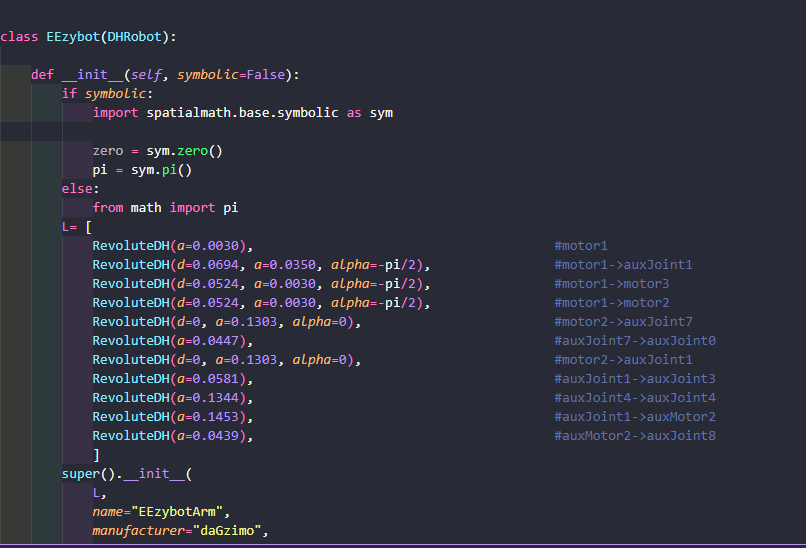
\includegraphics[scale=0.6]{img/dh.png}
		\end{center}
        \legend{\textbf{Fonte:} Autoria própria}
	\end{figure}

A descrição foi feita frame a frame, levando em conta todos os elos e juntas do robô. Por meio do método plot() é possivel visualizar um esboço dos elos e juntas do manipulador descrito (Fig. \ref{img:eezybot_dhcompleto.png}):

\imagem{0.6}{eezybot_dhcompleto.png}{EEzybotArm.plot() conforme foi descrito}{Autoria própria}

Com base no texto de \cite{Siciliano2009}, uma forma de analisar uma cadeia fechada é abrindo virtualmente a junta que une e fecha a cadeia, e analisar separadamente as duas cadeias que se formam, uma curta e outra longa.  Seguindo essa metodologia, outras formas de descrever o EEzybotArm no RTB foram pensadas e aplicadas, como visto nas figuras \ref{img:eezybot_dhshort} e \ref{img:eezybot_dhlong}. E ao descrever o manipulador essa forma, os plots dos manipuladores são gerados conforme as figuras \ref{img:eezybot_dhshort_plot} e \ref{img:eezybot_dhlong_plot}.

\begin{figure}[!htbp]
\centering
    \caption{\label{img:figura23} Parâmetros de DH do manipulador}
    \subcaptionbox{\label{img:eezybot_dhshort} DH para a cadeia curta do EEzybotArm}{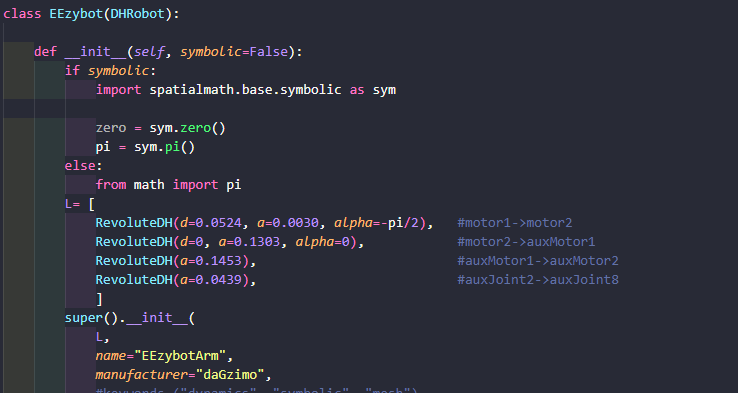
\includegraphics[scale=.5]{img/eezybot_dhshort.png}}
    \subcaptionbox{\label{img:eezybot_dhlong} DH para a cadeia longa do EEzybotArm}{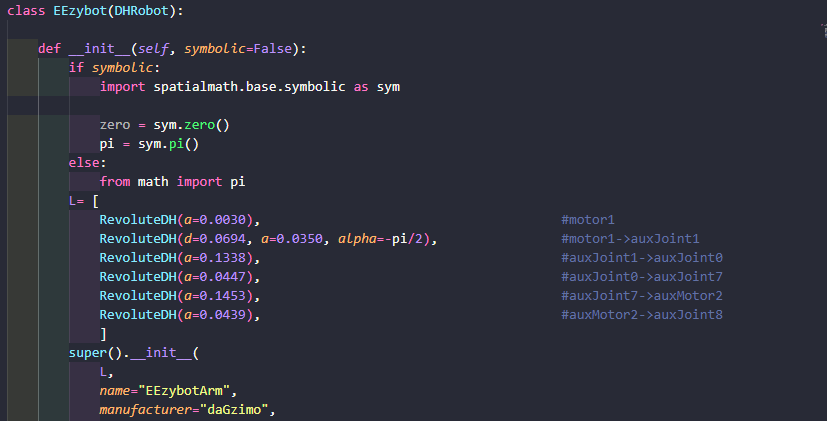
\includegraphics[scale=.5]{img/eezybot_dhlong.png}}
    \vspace{1.5em}
    \legend{\textbf{Fonte:} Autoria própria}
\label{fig:dag}
\end{figure}

\begin{figure}[!htbp]
\centering
    \caption{\label{img:figura23b} Parâmetros de DH do manipulador}
    \subcaptionbox{\label{img:eezybot_dhshort_plot} Plot para a cadeia curta do EEzybotArm}{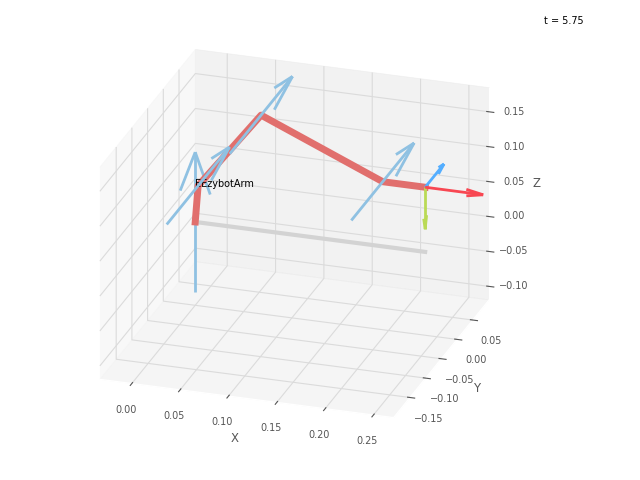
\includegraphics[scale=.55]{img/eezybot_dhshort_plot.png}}
    \subcaptionbox{\label{img:eezybot_dhlong_plot} Plot para a cadeia longa do EEzybotArm}{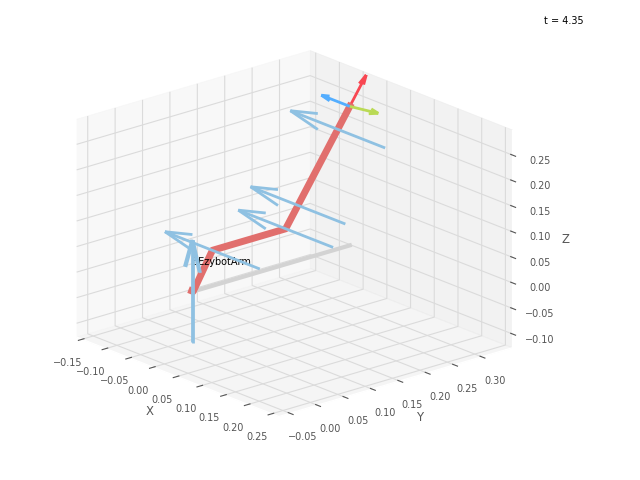
\includegraphics[scale=.55]{img/eezybot_dhlong_plot.png}}
    \vspace{1.5em}
    \legend{\textbf{Fonte:} Autoria própria}
\label{fig:dag}
\end{figure}

O repositório no Github easyEEZYbotArm do @meisben \cite{MoneyCoomes2021} disponibiliza um controlador python e arduino para o EEZYbotARM Mk1 e Mk2, incluindo cinemática nas três dimensões. Investigando os códigos, a função que implementa a cinemática inversa segue o método geométrico aplicado por \cite{costa2017}, chegando aos mesmos resultados. Então unindo o CoppeliaSim a esses scripts em python foi possível estabelecer uma comunicação satisfatória entre os dois ambientes (Fig. \ref{img:figura24.png}). Apenas as funções de cinemática inversa e plot foram utilizadas do projeto easyEEZYbotArm. 

\imagem{0.5}{figura24.png}{EEzybotArm: Plot no python e simulação no CoppeliaSim}{Autoria própria}



%--------------------------------------------------------------------------------------
% Insere a seção de cronograma
% Está comentada porque só é necessária no TCC I
%--------------------------------------------------------------------------------------
%\section{Cronograma TCC II}
%
%A continuidade desse projeto se dará da seguinte forma:
%\begin{itemize}
%	\item Com base no modelo CAD, os parâmetros de Denavit-Hartenberg serão obtidos, para
%então realizar a análise da cinemática direta e da cinemática inversa do manipulador;
%	\item As partes serão impressas, e o manipulador, montado;
%	\item O controle do manipulador será desenvolvido e implementado no arduino uno;
%	\item Testes e experimentos serão realizados a fim de comparar os resultados obtidos com
%os dados encontrados nas análises de cinemática;
%	\item Publicar os resultados em repositórios, a fim de compartilhar com a comunidade
%entusiasta do faça você mesmo dados cinemáticos e dinâmicos de um projeto tido
%como amador.
%\end{itemize}
%
%\newpage
%\section{Cronograma} \label{sec:crono}
%
%A tabela \ref{tab:cronograma} mostra o cronograma de atividades a serem executadas para o TCC II, com ênfase no calendário de 2022.1 da UNIVASF.
%
%\begin{table}[!thb]
	%\huge
	%\centering
	%\caption{\label{tab:cronograma} Cronograma das atividades previstas para o TCC II}
	%\begin{adjustbox}{max width=\textwidth}
		%\begin{tabular}{|l|l|l|l|l|l|}
			%\toprule
			%\textbf{Atividade}									& Out & Nov & Dez & Jan & Fev \\ \hline
		%	Analise Cinemática com RTB                          & x   & x   &     &     &     \\ \hline
		%	Montar manipulador impresso                         &     & x   & x   &     &     \\ \hline
	%		Modelagem do controlador e implementação no Arduino &     &     &     & x   &     \\ \hline
	%		Testes e simulações                                 &     &     &     & x   & x   \\ \hline
	%		Escrita do TCC II                                   & x   & x   & x   & x   & x   \\ \hline
	%		Defesa do TCC II                                    &     &     &     &     & x   \\ \hline
	%		\end{tabular}
%	\end{adjustbox}
%	\legend{\textbf{Fonte:} Autoria própria.}
%\end{table}


		\chapter{Resultados} \label{ch:RD}

Neste capítulo, são apresentados os resultados obtidos por meio das etapas de modelagem e controle do robô manipulador EEzybotArm, um manipulador com geometria em paralelogramo, utilizando as ferramentas CoppeliaSim, Robotics Toolbox for Python (RTB) e alternativas ao RTB.

\section{Modelagem no CoppeliaSim}
A modelagem do EEzybotArm no ambiente virtual do CoppeliaSim foi realizada com sucesso. Foram criados os componentes correspondentes às juntas e ao efetuador, refletindo o funcionamento básico do manipulador. As articulações foram configuradas para seguir os movimentos esperados, e as simulações confirmaram a fidelidade do modelo à realidade.

 No entanto, a tentativa de controle utilizando o RTB para manipular os ângulos das juntas no CoppeliaSim encontrou desafios. Embora a comunicação entre as plataformas tenha sido estabelecida com sucesso, o modelo do EEzybotArm no RTB não alcançou resultados satisfatórios (Fig. \ref{img:eezybot_dhcompleto.png} e Fig. \ref{img:eezybot_dhlong_plot}). Na figura \ref{img:eezybot_dhshort_plot} a representação visual assemelha-se com o real, porem essa limitação sugere que o RTB pode não ser a solução mais adequada para modelar manipuladores com cadeia fechada, pois falta meios de definir as juntas passivas, e descrever situações onde duas ou mais juntas existem muito próximas entre si, com seus eixos de rotação paralelos. Apesar de ser uma caixa de ferramentas poderosa, com funcionalidades robustas e fáceis de usar e resultados visualmente muito ricos, cadeias fechadas ainda não são suportadas por essa ferramenta. 

\section{Alternativas ao RTB}
Para contornar essa limitação, explorou-se alternativas, notadamente um controlador desenvolvido por @meisben \cite{MoneyCoomes2021} disponível no GitHub. Através deste controlador, baseado em Python e que também conecta-se com uma placa Arduino, foi possível calcular a cinemática inversa do EEzybotArm e transmitir os parâmetros das juntas para o CoppeliaSim via ZMQ. Os resultados dessa abordagem se mostraram positivos, com a simulação bem-sucedida (Fig. \ref{img:resultados.png}) e o cumprimento dos objetivos traçados, que eram a modelagem e simulação do braço robótico utilizando um controlador externo ao CoppeliaSim para cálculos de cinemática inversa. Diferentemente do RTB, essa solução é feita pelo método geométrico, ao passo que o RTB realiza a computação por meio de análise numérica pelas transformadas elementares. Houve certa discrepância entre a posição do órgão terminal no CoppeliaSim em comparação com o resultado da cinemática inversa no python (Fig. \ref{img:console.png}). Em outros testes foram encontrados os seguintes valores capturados pelas imagens (\ref{img:resultados3.png}, \ref{img:console3.png}, \ref{img:resultados4.png} e \ref{img:console4.png}).

\imagem{0.4}{resultados.png}{EEzybotArm: Plot no python e simulação no CoppeliaSim - Simulação 1}{Autoria própria}
\imagem{0.65}{console.png}{EEzybotArm: resultado apos calculo de IK e envio para o CoppeliaSim - Simulação 1}{Autoria própria}

\imagem{0.4}{resultados3.png}{EEzybotArm: Plot no python e simulação no CoppeliaSim - Simulação 2}{Autoria própria}
\imagem{0.65}{console3.png}{EEzybotArm: resultado apos calculo de IK e envio para o CoppeliaSim - Simulação 2}{Autoria própria}

\imagem{0.4}{resultados4.png}{EEzybotArm: Plot no python e simulação no CoppeliaSim - Simulação 3}{Autoria própria}
\imagem{0.65}{console4.png}{EEzybotArm: resultado apos calculo de IK e envio para o CoppeliaSim - Simulação 3}{Autoria própria}


Isso se dá, entre outras possíveis causas, é erros de ajuste inicial das juntas no Coppelia e calibragem. Outro fator que provoca movimentos inesperados é o próprio motor (engine) de simulação do CoppeliaSim, que tenta manter tudo junto, como definido pelas constrains (restrições) entre os \textit{dummy's} (tanto em código como definindo o \textit{dummy link type}). Mas pela forma que o braço se apresenta em comparação com o plot da função em python, a simulação foi positiva, sendo necessário apenas pequenas correções.


Consequentemente, a combinação de diferentes abordagens culminou na modelagem satisfatória e na operação eficaz do EEzybotArm no ambiente virtual do CoppeliaSim. A superação das limitações do RTB através da implementação de controladores alternativos validou a viabilidade de simular e controlar o manipulador com geometria em paralelogramo, realçando a importância de soluções integradas e adaptativas na pesquisa e desenvolvimento robótico.
\begin{comment}

\section{Seção de exemplo 1 - Códigos} \label{sec:resex1}

\subsection{Subseção de exemplo 1 - Inserindo trechos de códigos}
 
O nosso querido Leonardo Cavalcante providenciou um comando que deixa nossos trechos de códigos bonitinhos e gera um elemento pré-textual de Lista de Códigos. 

Os códigos são adicionados através do comando seguinte:

\textbackslash sourcecode\{ Descrição \}\{Label\}\{Linguagem\}\{Arquivo com extensão\}

Um exemplo pode ser visto no código \ref{cmd:cron} abaixo.

\sourcecode{Configuração do intervalo de execução no Script Agendador}{cron}{javascript}{cron.js}


\section{Seção de exemplo 2 - Listas} \label{sec:resex2}

\subsection{Subseção de exemplo 2 - Lista de itens} 

Existem alguns tipos de listas no Latex, iremos exemplificar a lista sem numeração (seção \ref{subsubsec:itemize}), a lista enumerada (seção \ref{subsubsec:enumerate}) e a lista mista (seção \ref{subsubsec:mista}). As listas podem ser encadeadas de diversas maneiras,
de acordo com a necessidade do autor.

\subsubsection{Subsubseção de exemplo 1 - Lista sem numeração} \label{subsubsec:itemize}

Este é um exemplo de lista sem numeração.

\begin{itemize}
	\item \textbf{Cadastrar usuário}

		\begin{itemize}
    		\item Atores
		    	\begin{itemize}
    		    	\item Usuário
		    	\end{itemize}

	    	\item Fluxo de eventos primário
			    \begin{itemize}
	    		    \item o usuário deve se cadastrar informando seu nome, \textit{e-mail} e senha;
		        	\item a API armazena os dados do usuário;
		    	    \item o usuário é liberado para realizar o \textit{login}.
			    \end{itemize}

    		\item Fluxo alternativo
			    \begin{itemize}
		    	   \item o usuário desiste de se cadastrar e cancela o caso de uso clicando no botão voltar.
	    		\end{itemize}

		\end{itemize}
	
\end{itemize}

\subsubsection{Subsubseção de exemplo 2 - Lista enumerada} \label{subsubsec:enumerate}

Este é um exemplo de lista enumerada.

\begin{enumerate}
	\item O Usuário deseja ver o histórico das variáveis climáticas, então através da interface de usuário escolhe o período ao qual o histórico se refere;
	\item A aplicação solicita à API através de uma requisição HTTP contendo o momento de início e o momento do fim do período em seus parâmetros;     			\item A API recebe a solicitação e se comunica com a base de dados, então requere as informações quem possuem a data de leitura no intervalo escolhido;
	\item A base de dados retorna os dados em formato Json para a API;
	\item A API responde à requisição retornando os dados, também em formato Json, para a aplicação cliente;
	\item A aplicação cliente renderiza os gráficos utilizando o conjunto de dados obtidos.
\end{enumerate}

\subsubsection{Subsubseção de exemplo 3 - Lista mista} \label{subsubsec:mista}

Este é um exemplo de lista mista.

\begin{itemize}
	\item \textbf{Cadastrar usuário}

		\begin{itemize}
    		\item Atores
		    	\begin{itemize}
    		    	\item Usuário
		    	\end{itemize}

	    	\item Fluxo de eventos primário
			    \begin{enumerate}
	    		    \item o usuário deve se cadastrar informando seu nome, \textit{e-mail} e senha;
		        	\item a API armazena os dados do usuário;
		    	    \item o usuário é liberado para realizar o \textit{login}.
			    \end{enumerate}

    		\item Fluxo alternativo
			    \begin{itemize}
		    	   \item o usuário desiste de se cadastrar e cancela o caso de uso clicando no botão voltar.
	    		\end{itemize}

		\end{itemize}

	\item \textbf{Visualizar dados atuais}

		\begin{itemize}
		    \item Atores
	    		\begin{itemize}
		    	    \item Usuário
			    \end{itemize}
    
	    	\item Pré-condições
			    \begin{itemize}
		     	   \item o usuário deve estar autenticado
			    \end{itemize}

	    	\item Fluxo de eventos primário
			    \begin{enumerate}
		    	    \item o usuário deve efetuar o \textit{login} informando o \textit{e-mail} e a senha;
	    		    \item caso o usuário não seja autenticado, o sistema informa a respeito de credenciais inválidas e encerra o caso de uso;
		    	    \item a API autentica o usuário;
    			    \item o usuário é liberado para visualizar os dados atuais dos sensores da estação;
		        	\item após a visualização o usuário pode finalizar o caso de uso ou efetuar uma nova consulta se desejar.
			    \end{enumerate}

    		\item Fluxo alternativo
			    \begin{itemize}
    			   \item o usuário desiste de visualizar os dados atuais e cancela o caso de uso clicando no botão voltar.
			    \end{itemize}

		\end{itemize}

	\item \textbf{Visualizar histórico}

		\begin{itemize}
		    \item Atores
	    		\begin{itemize}
		    	    \item Usuário
	    		\end{itemize}

	    	\item Pré-condições
    			\begin{itemize}
			        \item o usuário deve estar autenticado
			    \end{itemize}

		    \item Fluxo de eventos primário
			    \begin{enumerate}
			        \item o usuário deve efetuar o \textit{login} informando o \textit{e-mail} e a senha;
			        \item caso o usuário não seja autenticado, o sistema informa a respeito de credenciais inválidas e encerra o caso de uso;
			        \item a API autentica o usuário;
			        \item o usuário é liberado para escolher qual período cujo histórico será exibido;
			        \item o usuário seleciona as variáveis a serem exibidas no gráficos de linhas;
			        \item após a visualização do histórico o usuário pode finalizar o caso de uso se desejar.
			    \end{enumerate}

		    \item Fluxo alternativo
			    \begin{enumerate}
			        \item após a escolha do período de exibição do histórico o usuário pode voltar para a tela anterior e escolher um novo período;
			        \item o histórico é exibido para o usuário;
			        \item após a visualização do histórico o usuário pode finalizar o caso de uso ou efetuar uma nova consulta se desejar.
			    \end{enumerate}

		    \item Fluxo alternativo
			    \begin{enumerate}
			        \item o usuário desiste de visualizar o histórico e cancela o caso de uso clicando no botão voltar.
			    \end{enumerate}
		\end{itemize}
\end{itemize}

\end{comment}


		%--------------------------------------------------------------------------------------
% Este arquivo contém a sua conclusão
%--------------------------------------------------------------------------------------
\chapter{Considerações Finais e Trabalhos Futuros}

Neste trabalho, investigamos a modelagem e análise de um braço robótico do tipo EEzybotArm com geometria em paralelogramo, por meio da integração entre o CoppeliaSim e o Robotics Toolbox for Python (RTB), bem como alternativas complementares de controle. Ao final desta pesquisa, é possível traçar conclusões pertinentes e reflexões acerca dos resultados alcançados.

A modelagem do EEzybotArm MK2 no CoppeliaSim demonstrou ser eficaz, permitindo a representação acurada de suas juntas e funcionalidades básicas. No entanto, a tentativa de controle utilizando o RTB revelou limitações na modelagem de manipuladores com cadeia fechada (Fig. \ref{img:eezybot_dhcompleto.png} e Fig. \ref{img:eezybot_dhlong_plot}). Tal constatação ressalta a importância de considerar abordagens alternativas quando se depara com complexidades geométricas.

A busca por soluções eficazes levou-nos a explorar um controlador desenvolvido em Python, gentilmente disponibilizado por @meisben no GitHub e com base no modelo geométrico de \citeonline{costa2017}. Essa alternativa provou ser bem-sucedida, permitindo o cálculo da cinemática inversa e a transmissão de parâmetros das juntas para o CoppeliaSim via protocolo ZMQ. Essa abordagem ressalta a flexibilidade e a adaptabilidade como fatores cruciais na pesquisa em robótica, proporcionando soluções viáveis quando os métodos convencionais apresentam limitações.

Este estudo contribui para a compreensão das complexidades envolvidas na modelagem e análise de manipuladores robóticos com geometria em paralelogramo. A demonstração da eficácia de abordagens alternativas amplia as opções disponíveis para a simulação e controle de sistemas robóticos, mesmo diante de configurações mais desafiadoras. As lições aprendidas neste trabalho podem servir como base para pesquisas futuras na busca por soluções mais precisas e eficientes.

É importante ressaltar que, apesar dos avanços alcançados, este estudo enfrentou limitações, especialmente em relação à integração do RTB com manipuladores de cadeia fechada. Essa limitação sugere uma área de pesquisa promissora para o desenvolvimento de ferramentas mais abrangentes e eficazes, como o uso do pacote python TriP \cite{baumgartner2022trip}, voltado também para modelagem de estruturas rígidas. Além disso, a aplicabilidade dos resultados em cenários mais amplos da robótica e em contextos práticos também merece exploração adicional.

Em última análise, este trabalho ressalta que a robótica é um campo em constante evolução, onde a busca por soluções inovadoras e adaptativas é fundamental. A combinação de modelagem, simulação e abordagens alternativas de controle abre caminhos para avanços significativos e insights valiosos em um cenário tecnológico em constante mudança.


	\postextual
		\bibliography{tex/references}
		\bibliographystyle{abntex2-alf.bst}
        \chapter{Apêndice A} \label{apen:apendice1}


Os códigos a seguir foram desenvolvidos pelo autor com base em informações disponíveis na internet, como o manual de ajuda do CoppeliaSim e códigos de exemplo do Robotics ToolBox disponibilizados. O fluxo de mensagens trocadas pelo CoppeliaSim e o RTB é exemplificado na figura \ref{img:diagrama_codigo.png}; o fluxo geral do algoritmo da simulação envolvendo as duas ferramentas é visto na figura \ref{img:diagrama_fluxo_codigo.png}.

\imagem{0.8}{diagrama_codigo.png}{Fluxo de mensagens trocadas pelo CoppeliaSim e o RTB}{Fonte: Autoria própria}
\imagem{0.7}{diagrama_fluxo_codigo.png}{Fluxo geral do algoritmo da simulação}{Fonte: Autoria própria}


\newpage


\section{Codigo em Lua para controle da simulação no CoppeliaSim}
\sourcecodenolist{Server no CoppeliaSim}{server}{lua}{server.lua}
\sourcecodenolist{Client Python}{client}{python}{conection.py}
\sourcecodenolist{EEzybotArm DHModel - Completo}{dhmodel}{python}{eezybotDH_completo.py}
\sourcecodenolist{EEzybotArm DHModel - Cadeia Curta}{dhmodel_short}{python}{eezybotDH_simplificado.py}
\sourcecodenolist{EEzybotArm DHModel - Cadeia Longa}{dhmodel_long}{python}{eezybotDH_simplificado_chainL.py}

		%\begin{anexosenv}
\chapter{} \label{anex:anexo1}


\end{anexosenv}


\end{document}
